\subsection{Overview}
\begin{figure}[H]
    \centering
    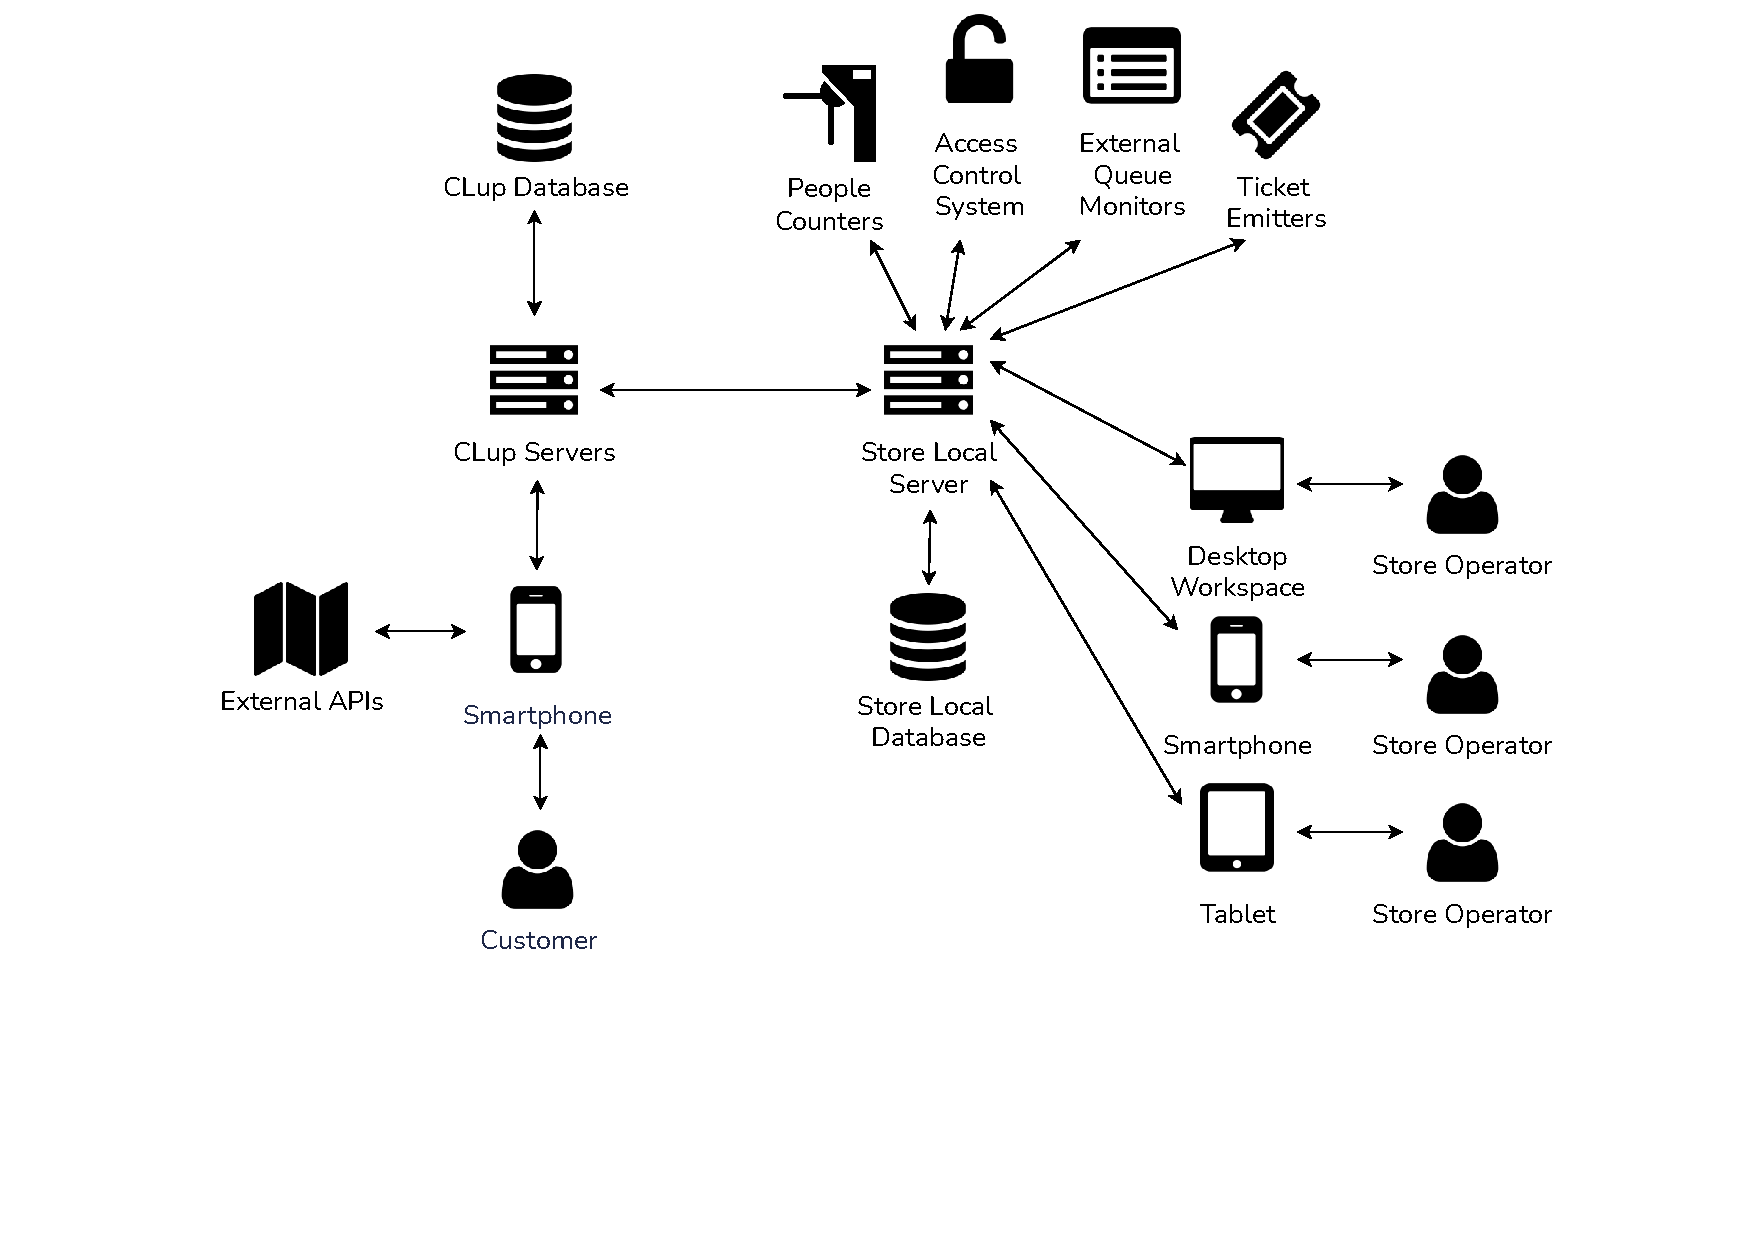
\includegraphics[scale=0.6]{Images/overview.pdf}
    \caption{\label{fig:Overview} CLup System Overview}
\end{figure}

This diagram shows the CLup system as a whole, its actors and main components, from an high level perspective. 

Store customers interact with the system by using a smartphone, which depends on external third party APIs to visualize and interact with maps.
Store operators can interact with the system using different kinds of devices, to better suit their needs when working at the shop: smartphones can be handy when they need to check information about the store queue while moving through departments; tablets make looking at graphs and statistics more easily without loosing the 'mobile' factor, and having a CLup application also on desktops can also be convenient for operators working at a desk (without having to switch from one device or another in their workflow).

CLup Customer Application communicates directly with CLup servers through REST APIs, while CLup Operator Application connects to the Store Local Server which retrieves data both from the Store Local Database and from CLup Servers. 

Store Devices also connect to the Store Local Server, to enhance the functionalities and automate tasks such as admitting customer entrances, monitoring the people inside the store departments, handing out tickets.

CLup Servers on the other hand only store data that is needed to permit queue regulations, for example information about occupancy limits, live occupancy of the stores, markets locations.

Following sections will analyze every major component more deeply, describing in detail its underlying sub-components and interfaces.  

\subsection{Component View}
\begin{figure}[H]
    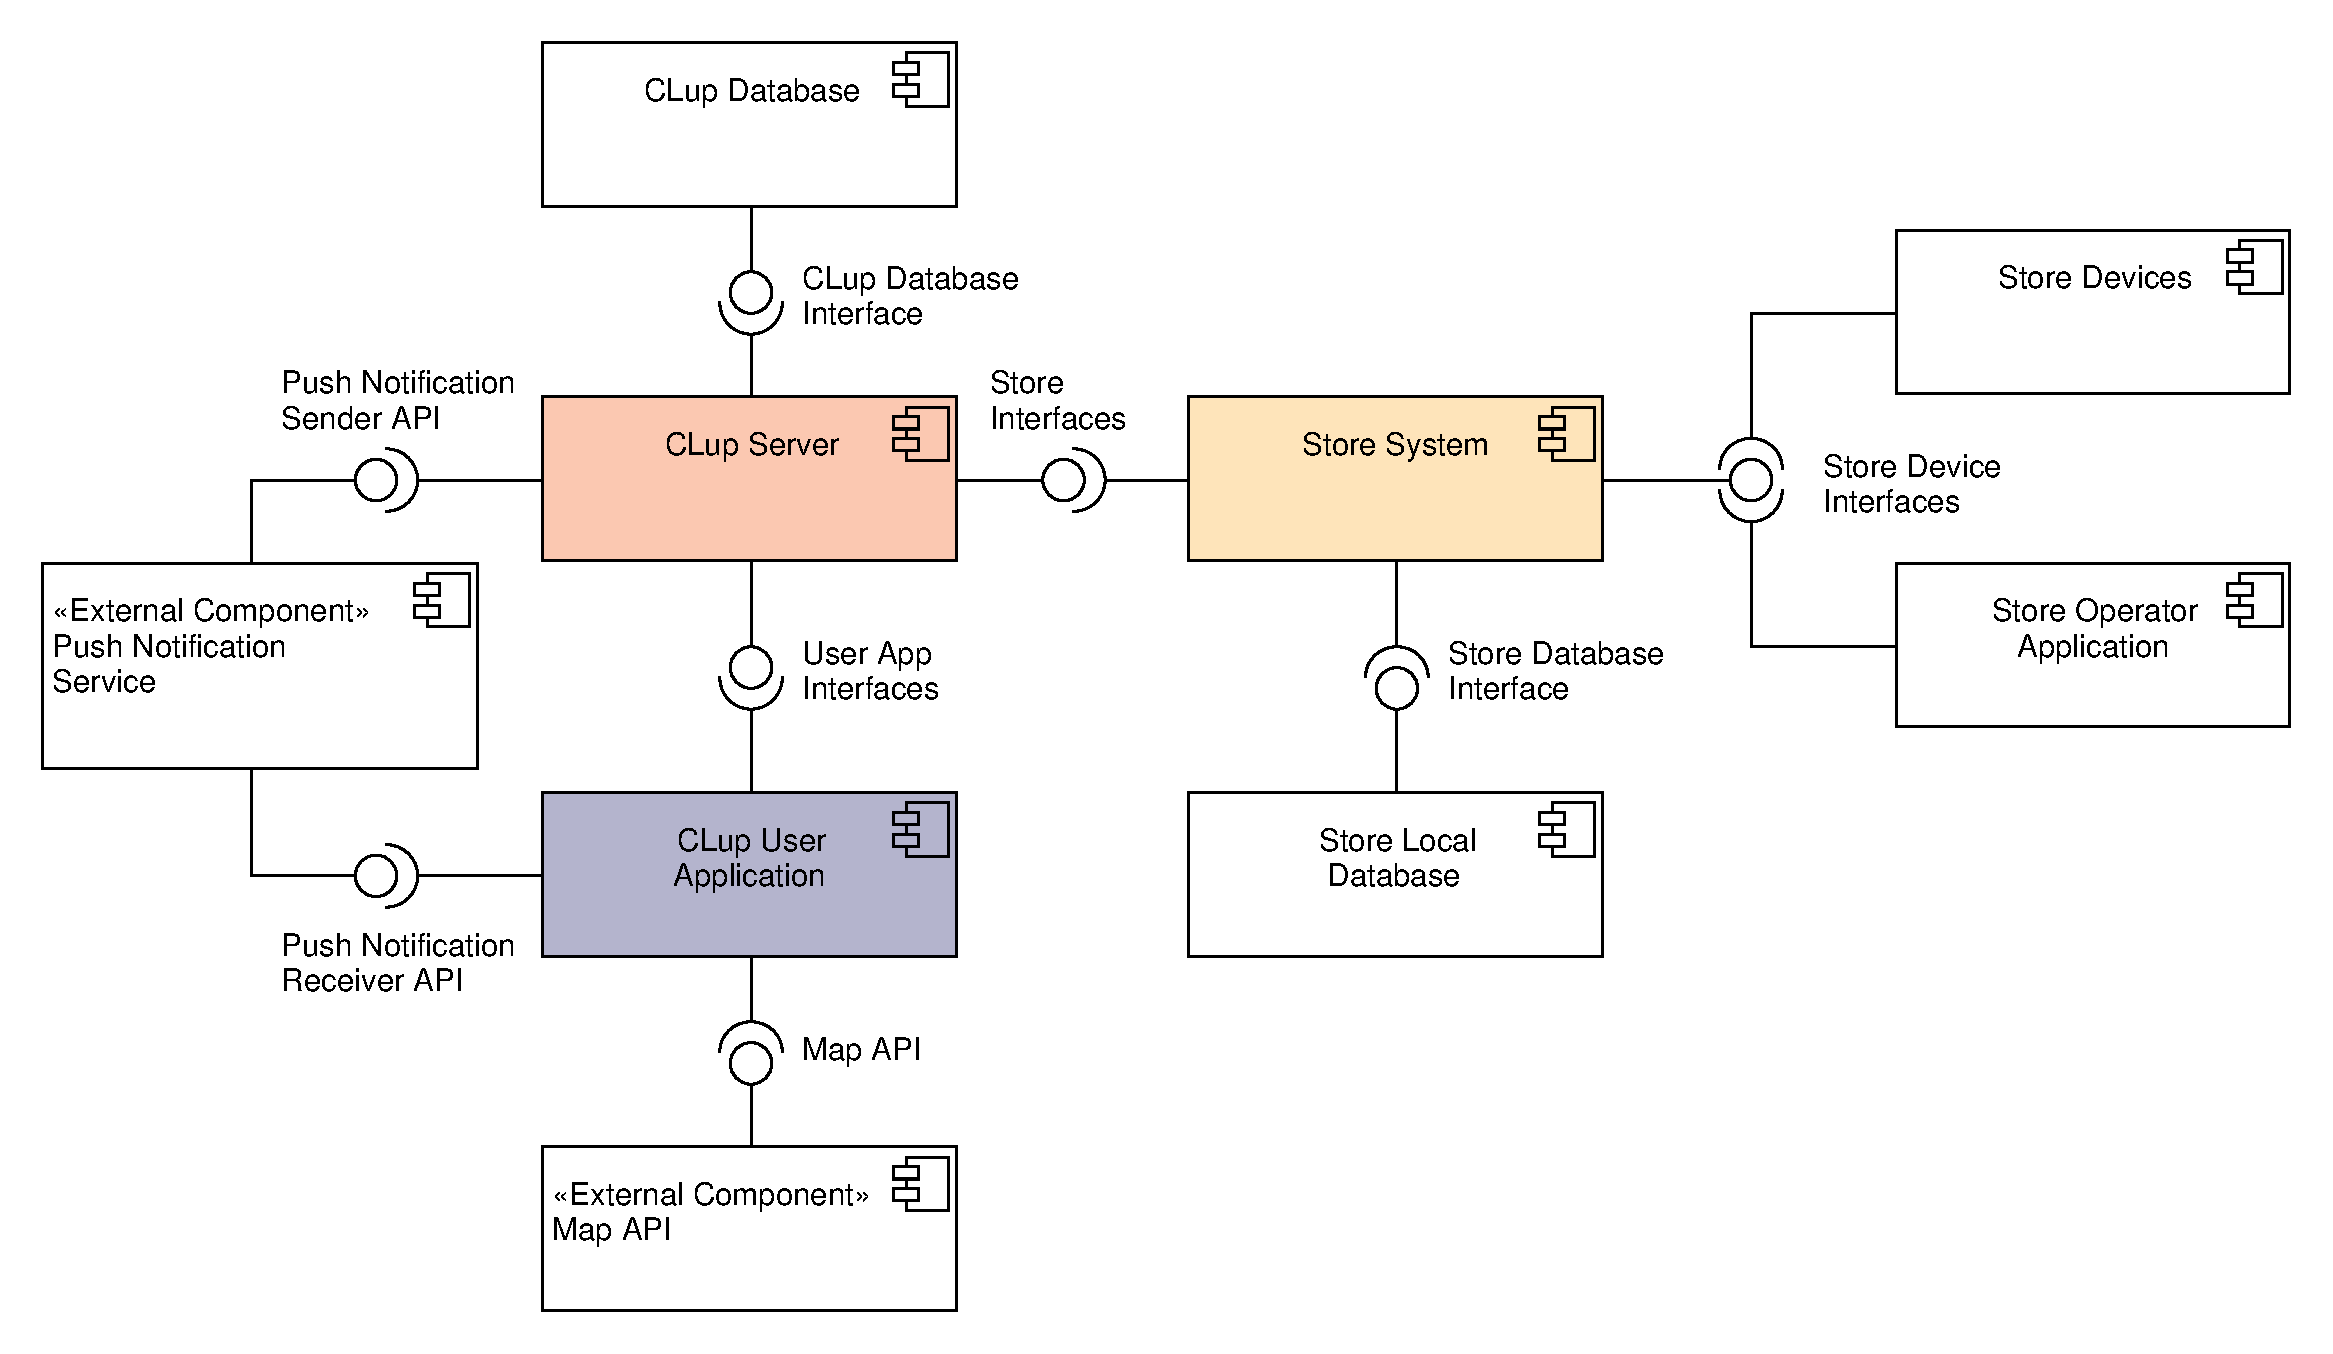
\includegraphics[width=\textwidth]{Images/UML_general_component.pdf}
    \caption{\label{fig:UML_comp_general}General component diagram}
\end{figure}
Figure~\ref{fig:UML_comp_general} shows a general, simplified, component view of the S2B.
The three main components of the system are: the CLup User Application, the CLup Server and the Store System with their databases. CLup system also interacts with external components like Map API Services and other physical components (i.e.~store devices).

Customers use the \textbf{CLup User application} to check supermarkets near them and eventually book a visit or retrieve a ticket. The User application interfaces with the \textbf{CLup server}. 

Sometimes the customer need to receive notifications about their ticket, to allow this the CLup Server and the application need to use the Push Notification service, each OS manufacturer provide his different push notification service. This service provides its dedicated API for sending and receiving push notifications.

The CLup server is the central component of the system, mediating between the customers and the stores. It manages customer authentication, tickets issued remotely by the CLup application, and hands out to the public information about stores to the customers (i.e.~opening hours, waiting times, etc). 

The \textbf{Store system} provides an interface for all the physical devices in the store, collecting and processing data from them and then routing the data to the CLup server or keeping it in the local database. The system communicates with a local database to store temporary data about tickets, the statistics collected and the authentication details of the store operators.

\subsubsection{CLup Server component view}
\begin{figure}[H]
    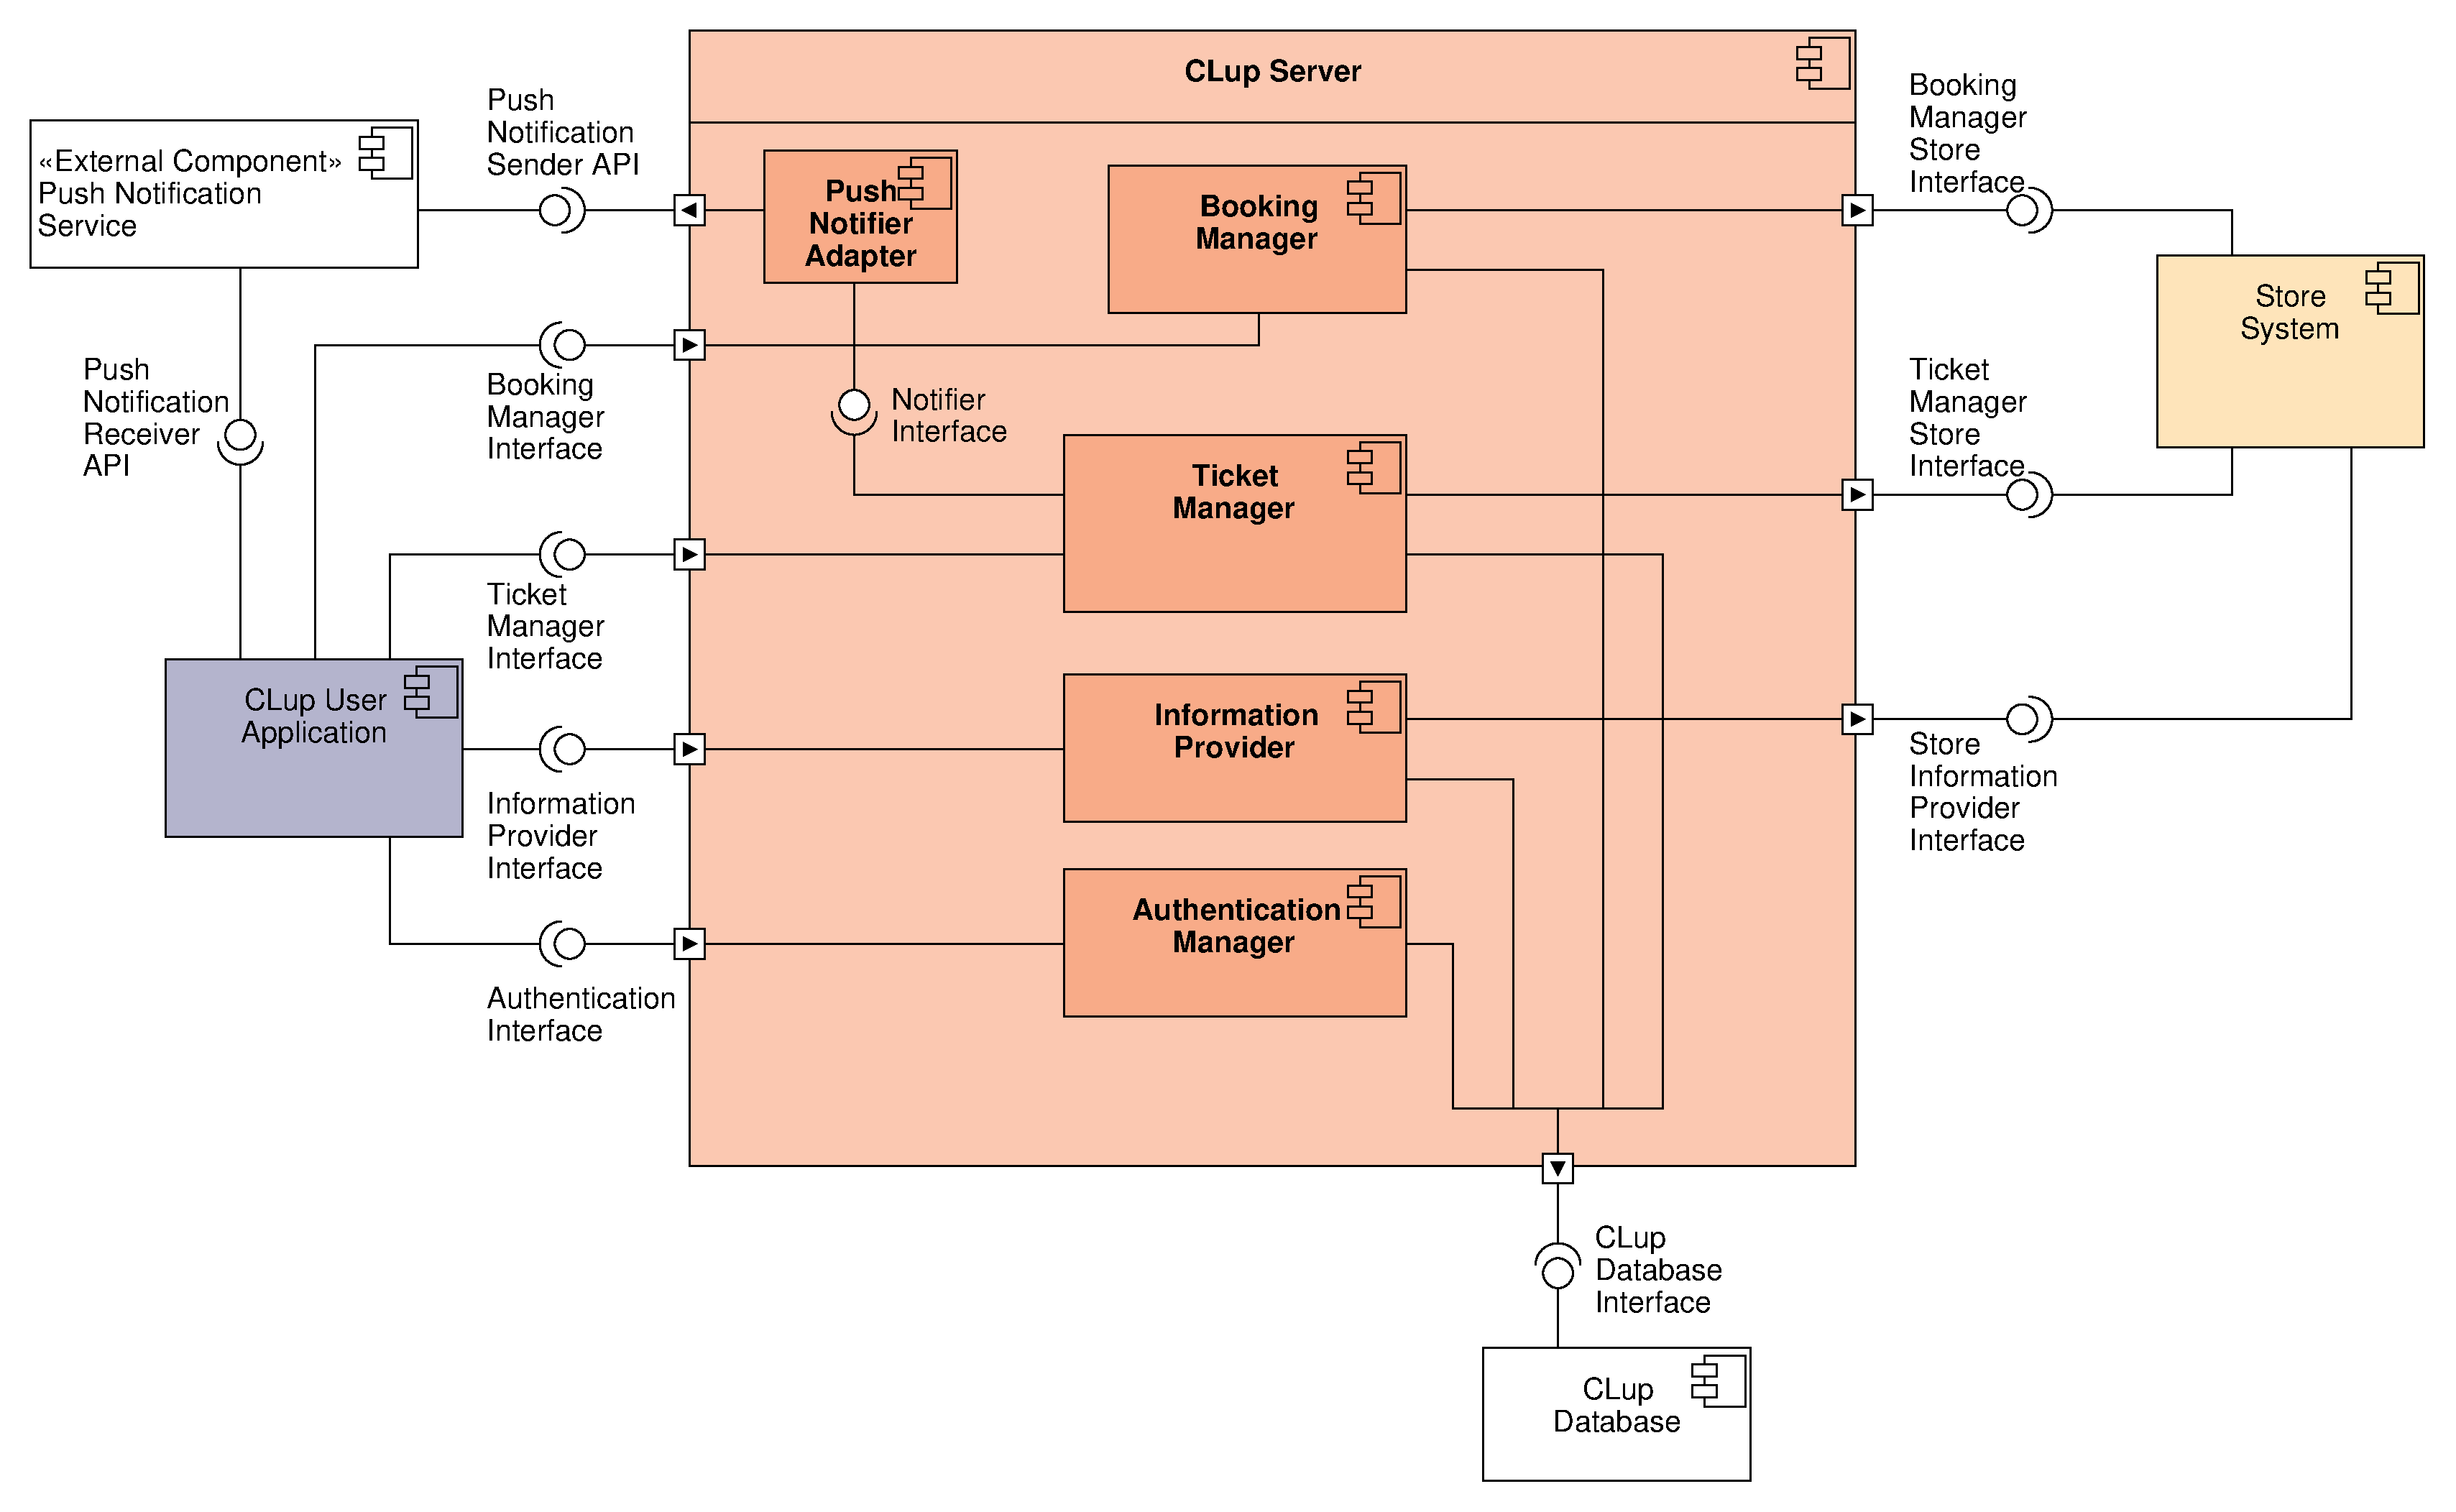
\includegraphics[width=\textwidth]{Images/UML_server_component.pdf}
    \caption{\label{fig:UML_comp_Clup_server}Component diagram for CLup server}
\end{figure}

The CLup server provides interfaces to the CLup User application and to each Store System. This component stores the persistent data in the CLup Database component communicating with it using a common Database interface.

The CLup Server has these internal components:
\begin{itemize}
    \item \textbf{Authentication Manager}: handles customer registration and authentication. To do this task this component needs to communicate tightly with the CLup database which stores the user data and their hashed passwords;
    \item \textbf{Information Provider}: hands out information to the customers requesting them. These information can be of various nature, like opening hours or the store crowdedness in various times of the day. This data is retrieved from the CLup database or from the Store System which uses another interface to push them periodically.
    \item \textbf{Ticket Manager}: issues virtual tickets when customers requests them. This component interfaces directly with the Store System, adding the created tickets to the queue. The component has the responsibility to notify the customers when it's time to approach the store entrance; it uses the notification interface, provided by the Notifier component.
    \item \textbf{Booking Manager}: handles the visit booking. Queries the database about free slots in the day when a customer wants to make a reservation. Requests are eventually finalized by attaching the shop list to the booking if and when the customer adds it from the application. This components also pushes updates to the Store System about changes regarding the bookings (e.g.~cancellation, shopping list changes, etc).
    \item \textbf{Push Notification Adapter}: handles all the aspects about sending push notifications to the users, taking into account that the CLup application can be running on different operating systems and that they provide different services to receive these notifications. The notifier needs to communicate with the external Push Notification Service, using the interface provided by that service.
\end{itemize}

\subsubsection{CLup customer application component view}
\begin{figure}[H]
    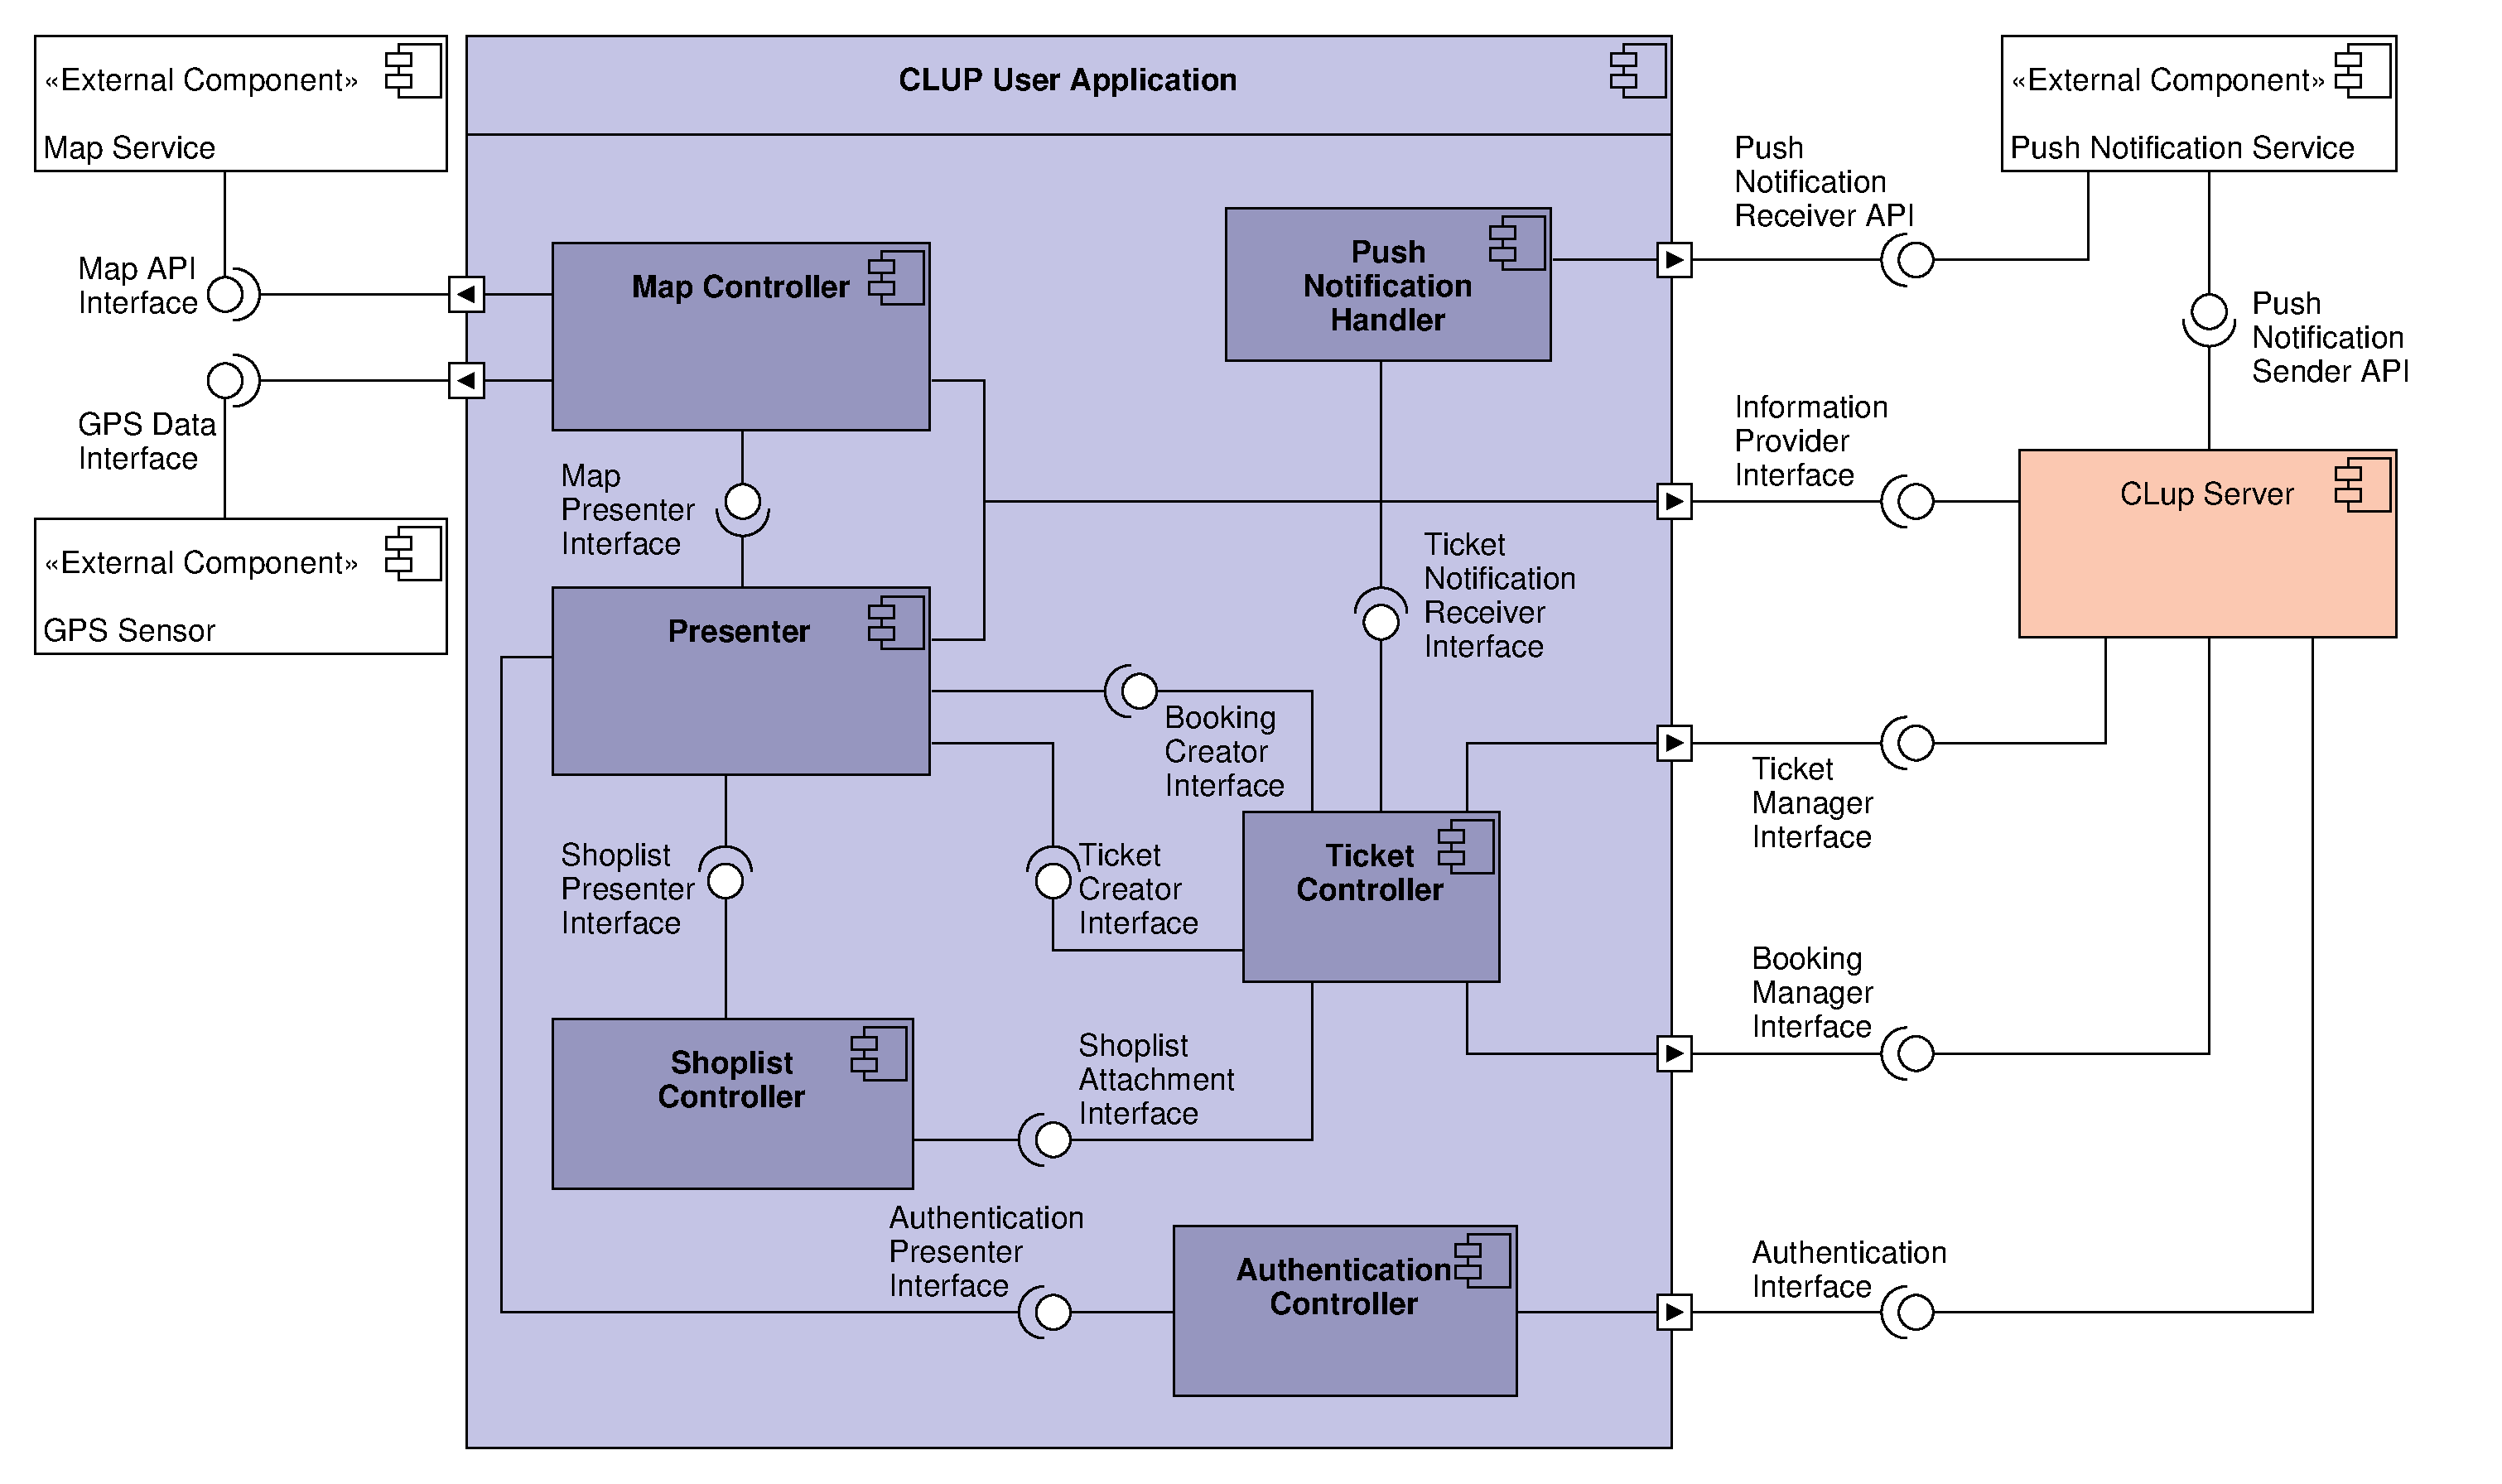
\includegraphics[width=\textwidth]{Images/UML_user_app_component.pdf}
    \caption{\label{fig:UML_comp_CLup_user_app}Component diagram for CLup User Application}
\end{figure}

The CLup user application provides the functionalities of CLup to store's customers. The applications needs to interface with the GPS Sensors and to an external map service that provides a map containing all the stores. The application also needs some controllers that will communicate with the CLup server to retrieve store information, authenticate, book a visit or create a queue ticket.

The user application contains these sub-components:
\begin{itemize}
    \item \textbf{Authentication}: allows the user to create a CLup account and to log-in with an existing account.
    \item \textbf{Map Controller}: Handles the communication with the external Map Service and the GPS. Exploits the Map API provided from the Map Service to get the map data near the user position then will request data to the CLup server in order to populate the map with the nearby stores.  access data about the location of the user. For this task the component will use the Information Provider Interface offered by the CLup server component.
    \item \textbf{Presenter}: Handles the GUI of the applications and the events from the user like the push of a button or the text boxes. Needs to relate with all the controllers components that handle different the different aspects and functionality of the application. To do this these component will provide their interface exposing all the functionalities that each controller offers.
    \item \textbf{Shop-list Controller}: manages the creation of shop lists that will be attached to visit bookings in order to estimate the occupancy of the various department of the store.
    \item \textbf{Push Notifications Handler}: handles and displays to the user the push notification received from the CLup Server about the bookings or the tickets created from the user. This component is provided by the underlying Operating System, and the interface is accessible through standard libraries of the application programming language.
\end{itemize}

\subsubsection{Store System component view}
\begin{figure}[H]
    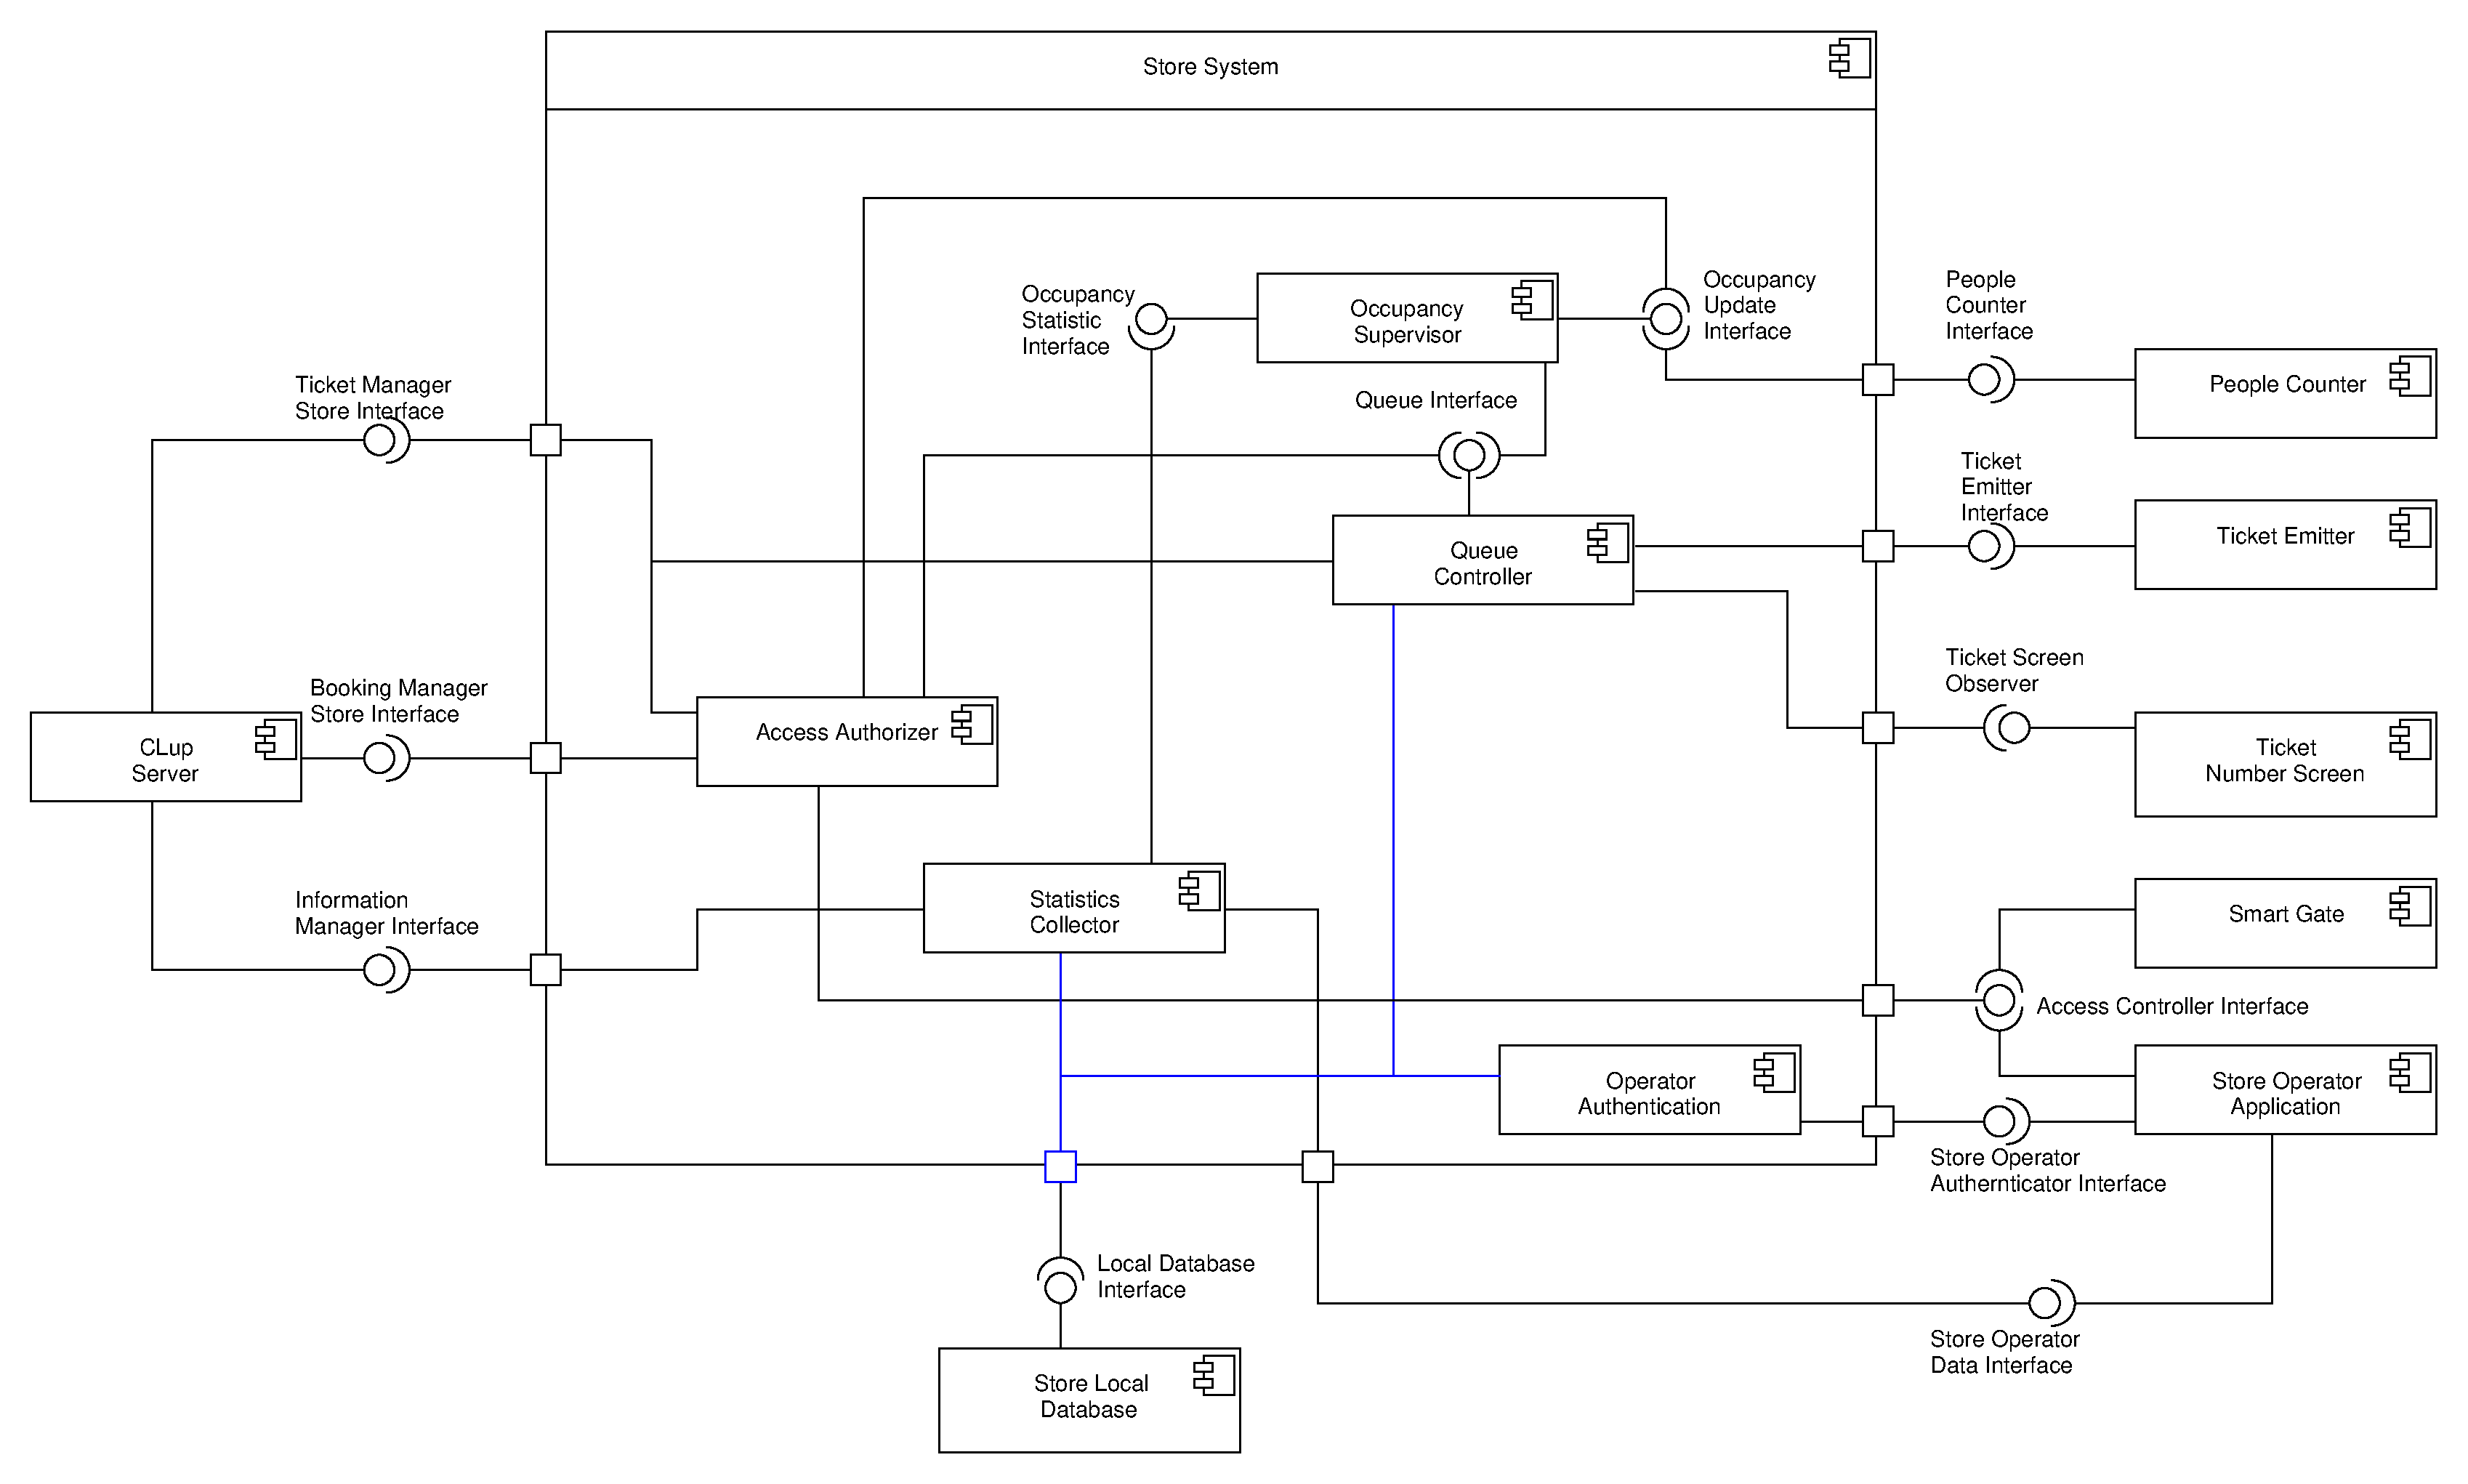
\includegraphics[width=\textwidth]{Images/UML_store_system_component.pdf}
    \caption{\label{fig:UML_comp_CLup_store_system}Component diagram for Store system}
\end{figure}

The Store System receives data from the store physical devices and combines it with the information retrieved by the CLup Servers. This component uses the interfaces provided by the CLup Server and lays out its own interfaces that are used by the physical devices located in the store. This component interfaces with a local database containing store statistics, store operators authentication data and local data that need persistency.

\begin{itemize}
    \item \textbf{Operator Authentication}: allows store operators to authenticate using their store credential. This component communicates with the Store Operator Application, which is used to manually check tickets and register the customer admissions in the store. The component fetches the authentication data in the store local database, using the interface provided by the database.
    \item \textbf{Occupancy Supervisor}: checks that the occupancy limits are not violated using all the data that it receives about people entering and leaving the store. This data can be provided directly by devices like People Counters, or from the Access Authorizer. The latters increments the counter of the number of people inside the store when an access is authorized. The Occupancy Supervisor checks information about the bookings and notifies the Queue Controller when there is space to admit new customers with a numbered ticket (without a booked visit).
    \item \textbf{Queue Controller}: handles the queueing of the customers by combining the data about virtual numbered tickets and paper numbered tickets, using the proper interfaces to communicate with the CLup Server. The Queue Controller is notified by the Occupancy Supervisor when customers in line can be called to the entrance; it then updates the ticket numbers on the screen placed at the store entrance (with the new numbers obtained using its interface).
    \item \textbf{Access Authorizer}: receives the code read by the Access Controller (that can be either a Smart Gate or a store operator), checks if that code is valid and allowed to enter, then notifies back the Access Controller. Even if the ticket is valid, before admitting a customer, this component needs to check that the occupancy limits of the store will not be violated by letting customer inside the store, consulting the Occupancy Supervisor. The Access Authorizer will check (requesting information from the CLup server) if the ticket refers to a pre-booked ticket; otherwise it will check if the ticket is on top of the queue using the Queue Controller interface.
    \item \textbf{Statistics Collector}: collects and periodically elaborates statistics with data from the Occupancy Supervisor and Queue Controller. Statistics are saved in the store local database. Brief elaborated data that can be shown to the customer (i.e.~indications of the crowdedness of the store, estimated waiting times,\ldots) are sent periodically to the CLup Server using the Store Information Provider interface.
\end{itemize}
\subsection{Deployment View}
\clearpage
\subsection{Runtime View}
The aim of the following sequence diagrams is to show how the components (the actors in the diagrams) interact between them at runtime. 
\begin{figure}[H]
    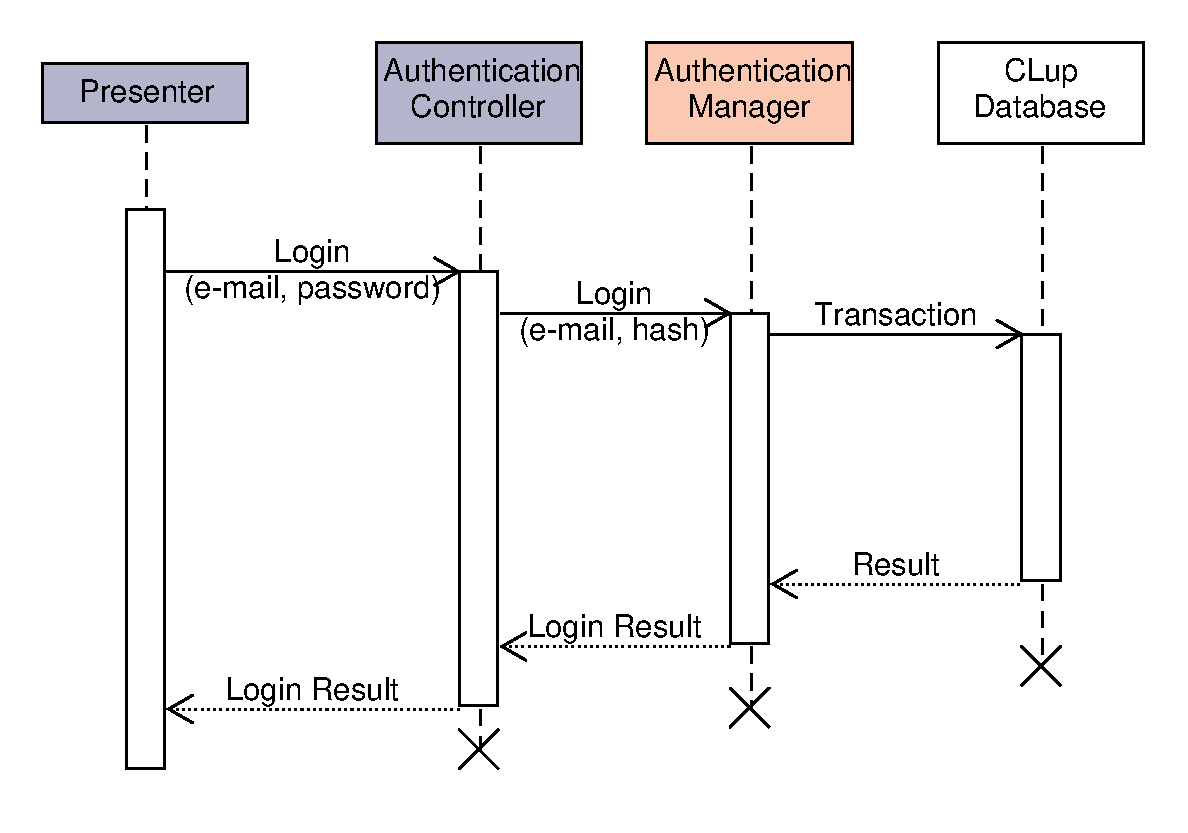
\includegraphics[width=\textwidth]{Images/UML_login_sequence.pdf}
    \caption{\label{fig:UML_login_sequence}User logs into CLup user application, runtime view}
\end{figure}
The diagram shown in Figure~\ref{fig:UML_login_sequence} describes the behavior of the system when the user request to login on CLup User Application\footnote{UC2 - Customer/Operator Authentication, refer to RASD}. The Authentication controller calls the Authentication manager that will check in the CLup database if the credential are correct, allowing the login.

\begin{figure}[H]
    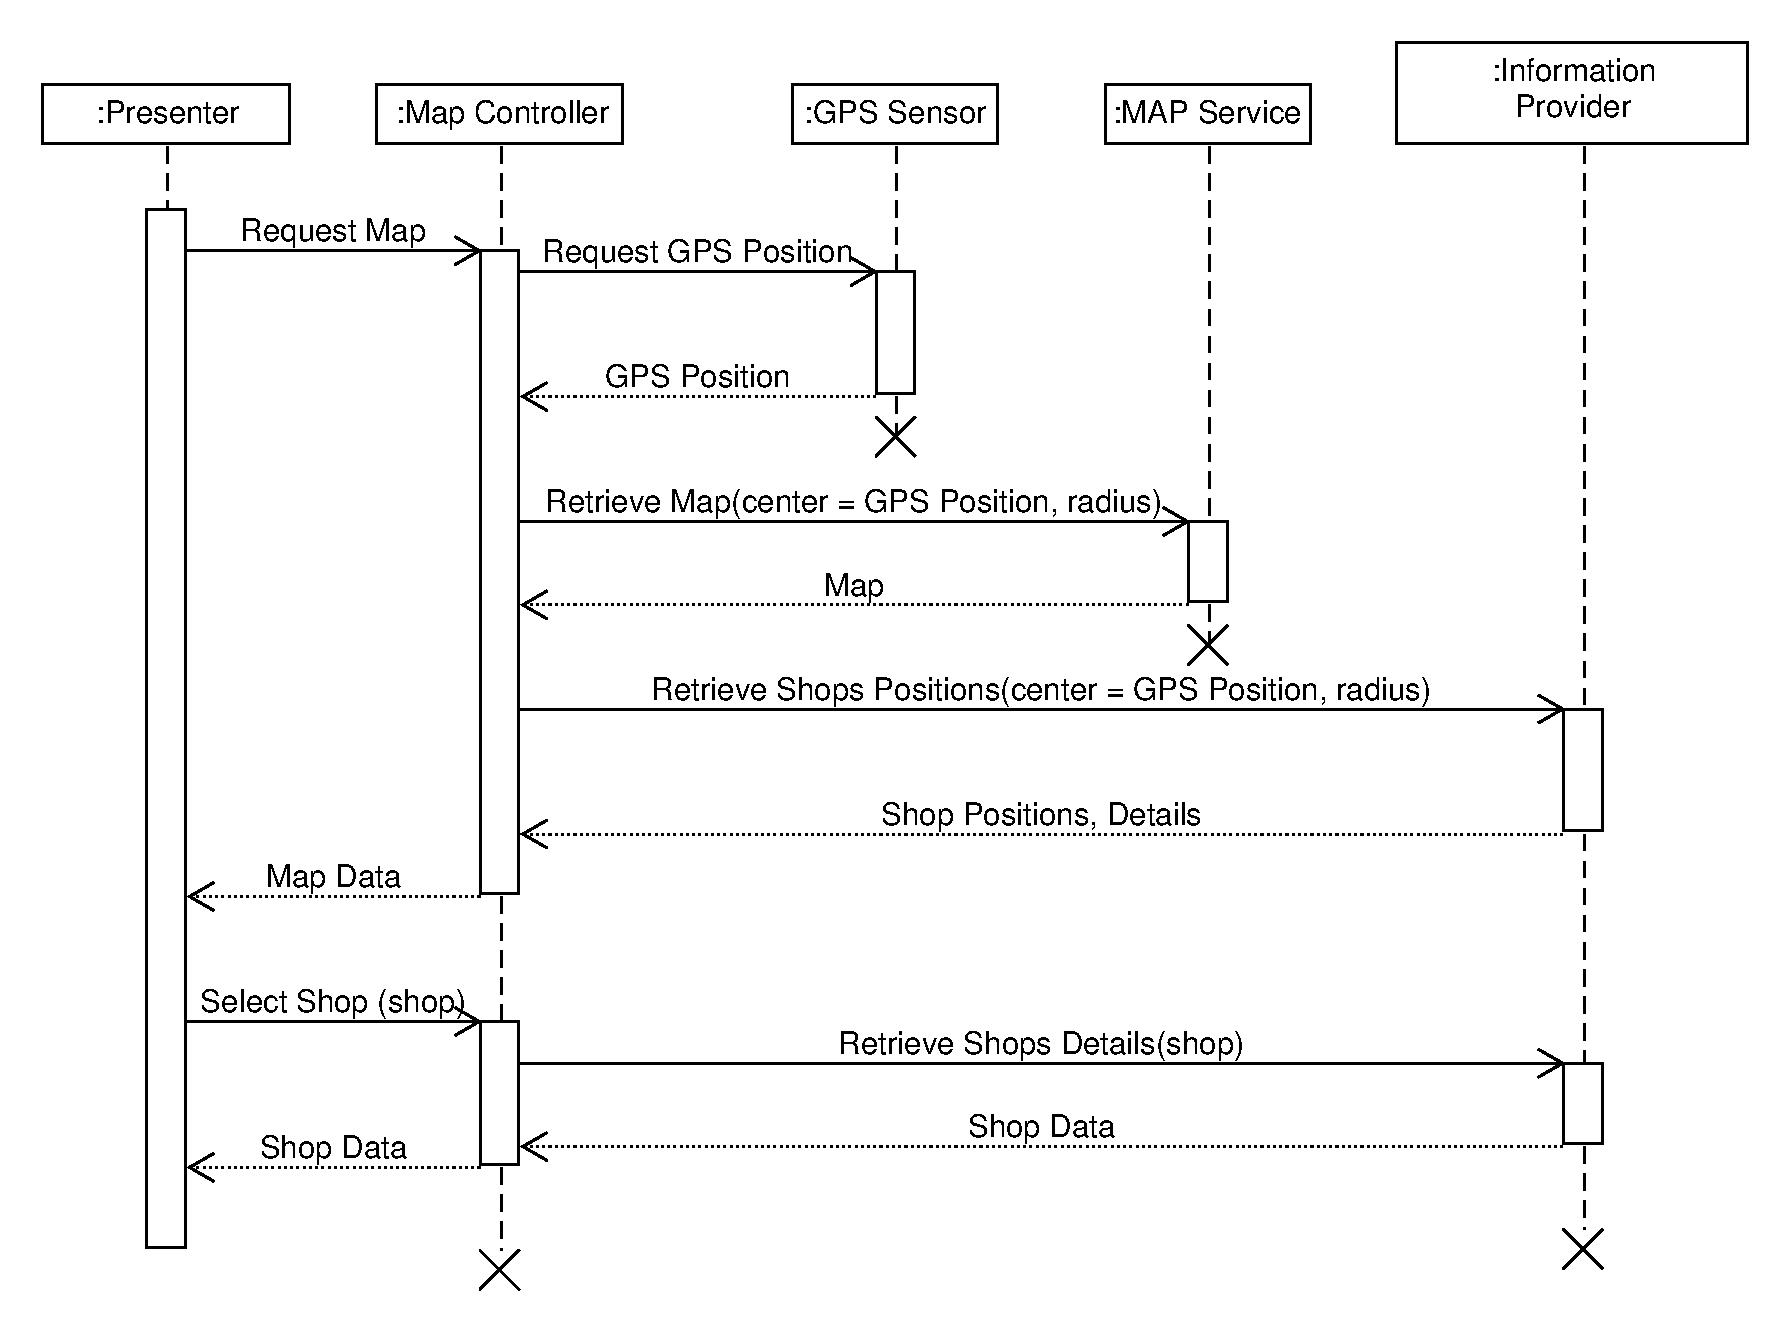
\includegraphics[width=\textwidth]{Images/UML_user_map_sequence.pdf}
    \caption{\label{fig:UML_user_map_sequence}User searches for a store in the map, runtime view}
\end{figure}
The diagram in Figure~\ref{fig:UML_user_map_sequence} shows how the system loads the map of all stores and shows it to the user\footnote{UC3 - Customer searches for the store page, refer to RASD}.

To determine which part of the map to load, the system needs to acquire the user position consulting the GPS sensor external component (external from the CLup system view, but built in most smartphones). The MAP API is then called to get the map data; concurrently a call to the Information Provider has to be done in order to get the positions and the basic information of all the stores to show in the map. When the Map Controller has all the data at its disposal, the map can finally be rendered by the Presenter. 

\begin{figure}[H]
    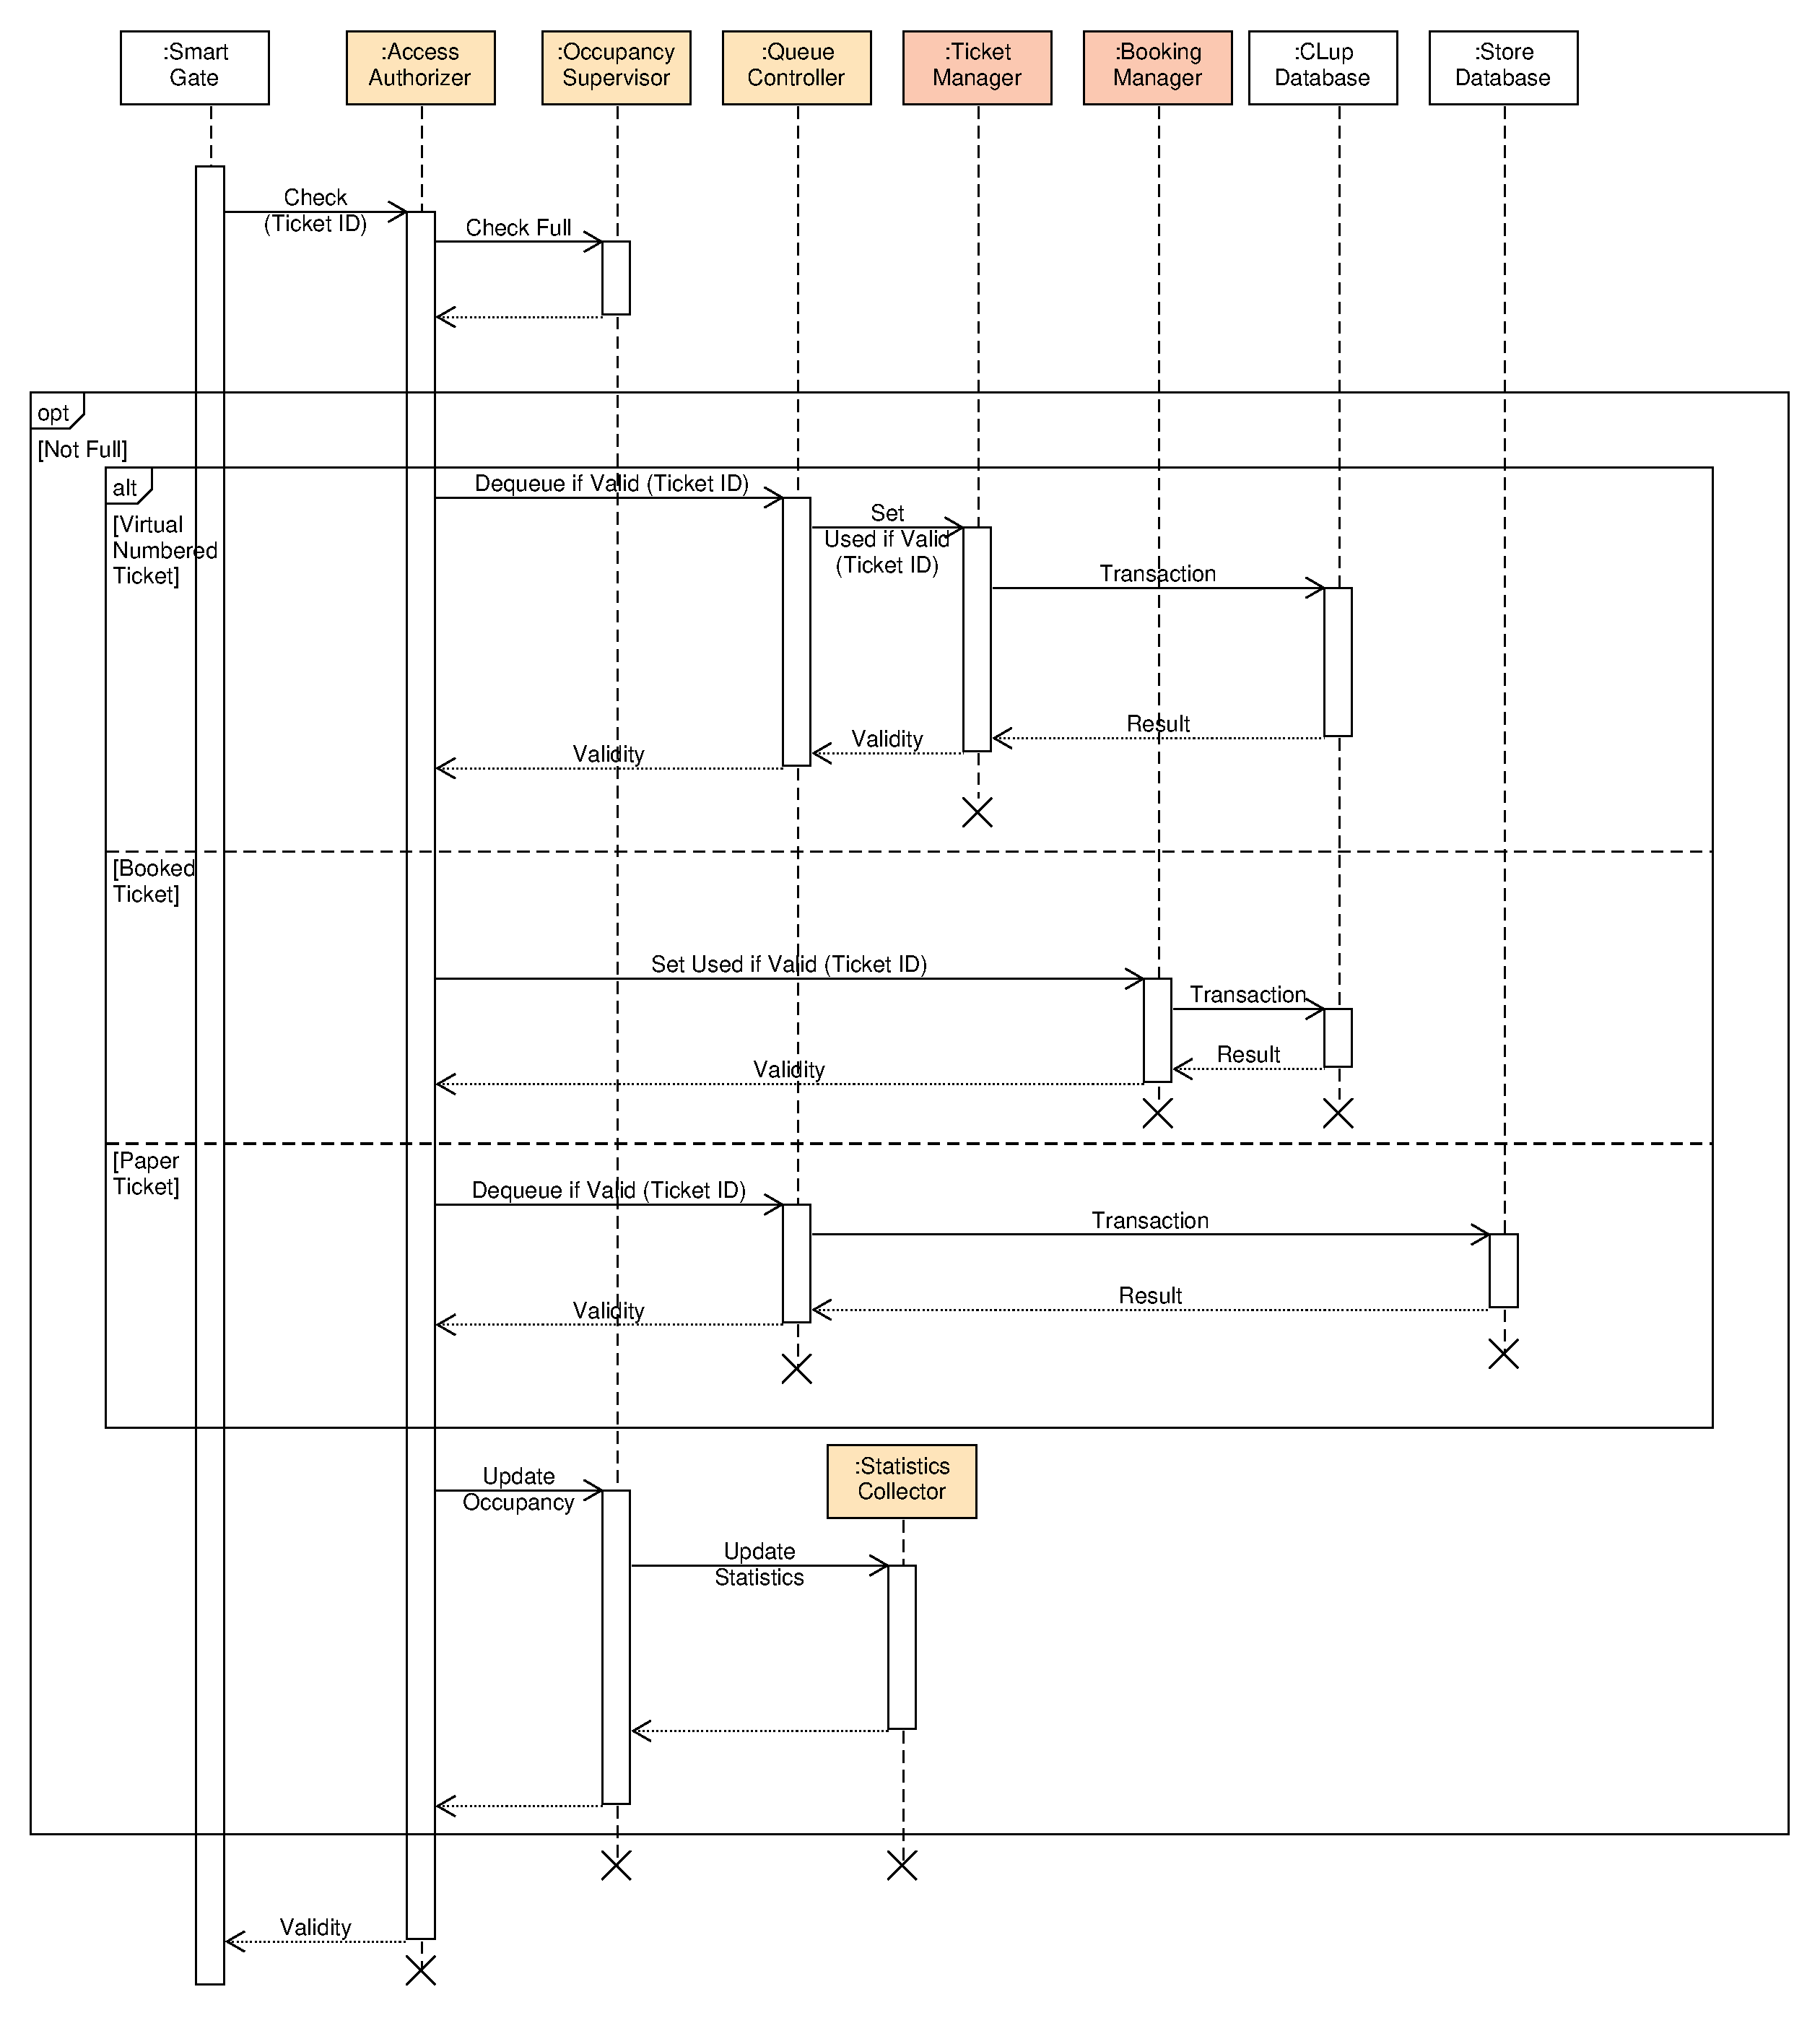
\includegraphics[width=1.1\textwidth]{Images/UML_ticket_scan_sequence.pdf}
    \caption{\label{fig:UML_ticket_scan_sequence}User scans a ticket to the access controller, runtime view}
\end{figure}
The diagram shown in Figure~\ref{fig:UML_ticket_scan_sequence} shows how the system behaves when a ticket is scanned\footnote{UC10 - Customer scans the ticket through an access control system to enter, refer to RASD}. The Access Authorizer receives the Ticket ID scanned by a Smart Gate (or an Operator). Before checking if the ticket ID exists and is valid, the store live occupancy is checked. If the supermarket is full the entrance can be denied (based on the supermarket policies). 

Then the Access Authorizer figures from the ID which type of ticket has been scanned; this could be achieved, for example, by reserving a digit of the ticket ID to differentiate ticket types.
Depending on the ticket type different actions are carried out:
\begin{itemize}
    \item Virtual Numbered Ticket: if the ticket is valid it is removed from the store queue and the ticket status is set to Inside Shop\footnote{RASD, Section 2.4 - Product Functions} on the CLup main database
    \item Booked Ticket: the Booking Manager is in charge of checking if the ticket is valid at the time of the scan
    \item Paper Ticket: if the ticket is valid it is removed from the store queue and its status is set to Inside Shop on the CLup main database
\end{itemize}

After this, the Occupancy Supervisor is called again and updates the people count, then the Access Controller grants the customer the access to the store.
\begin{figure}[H]
    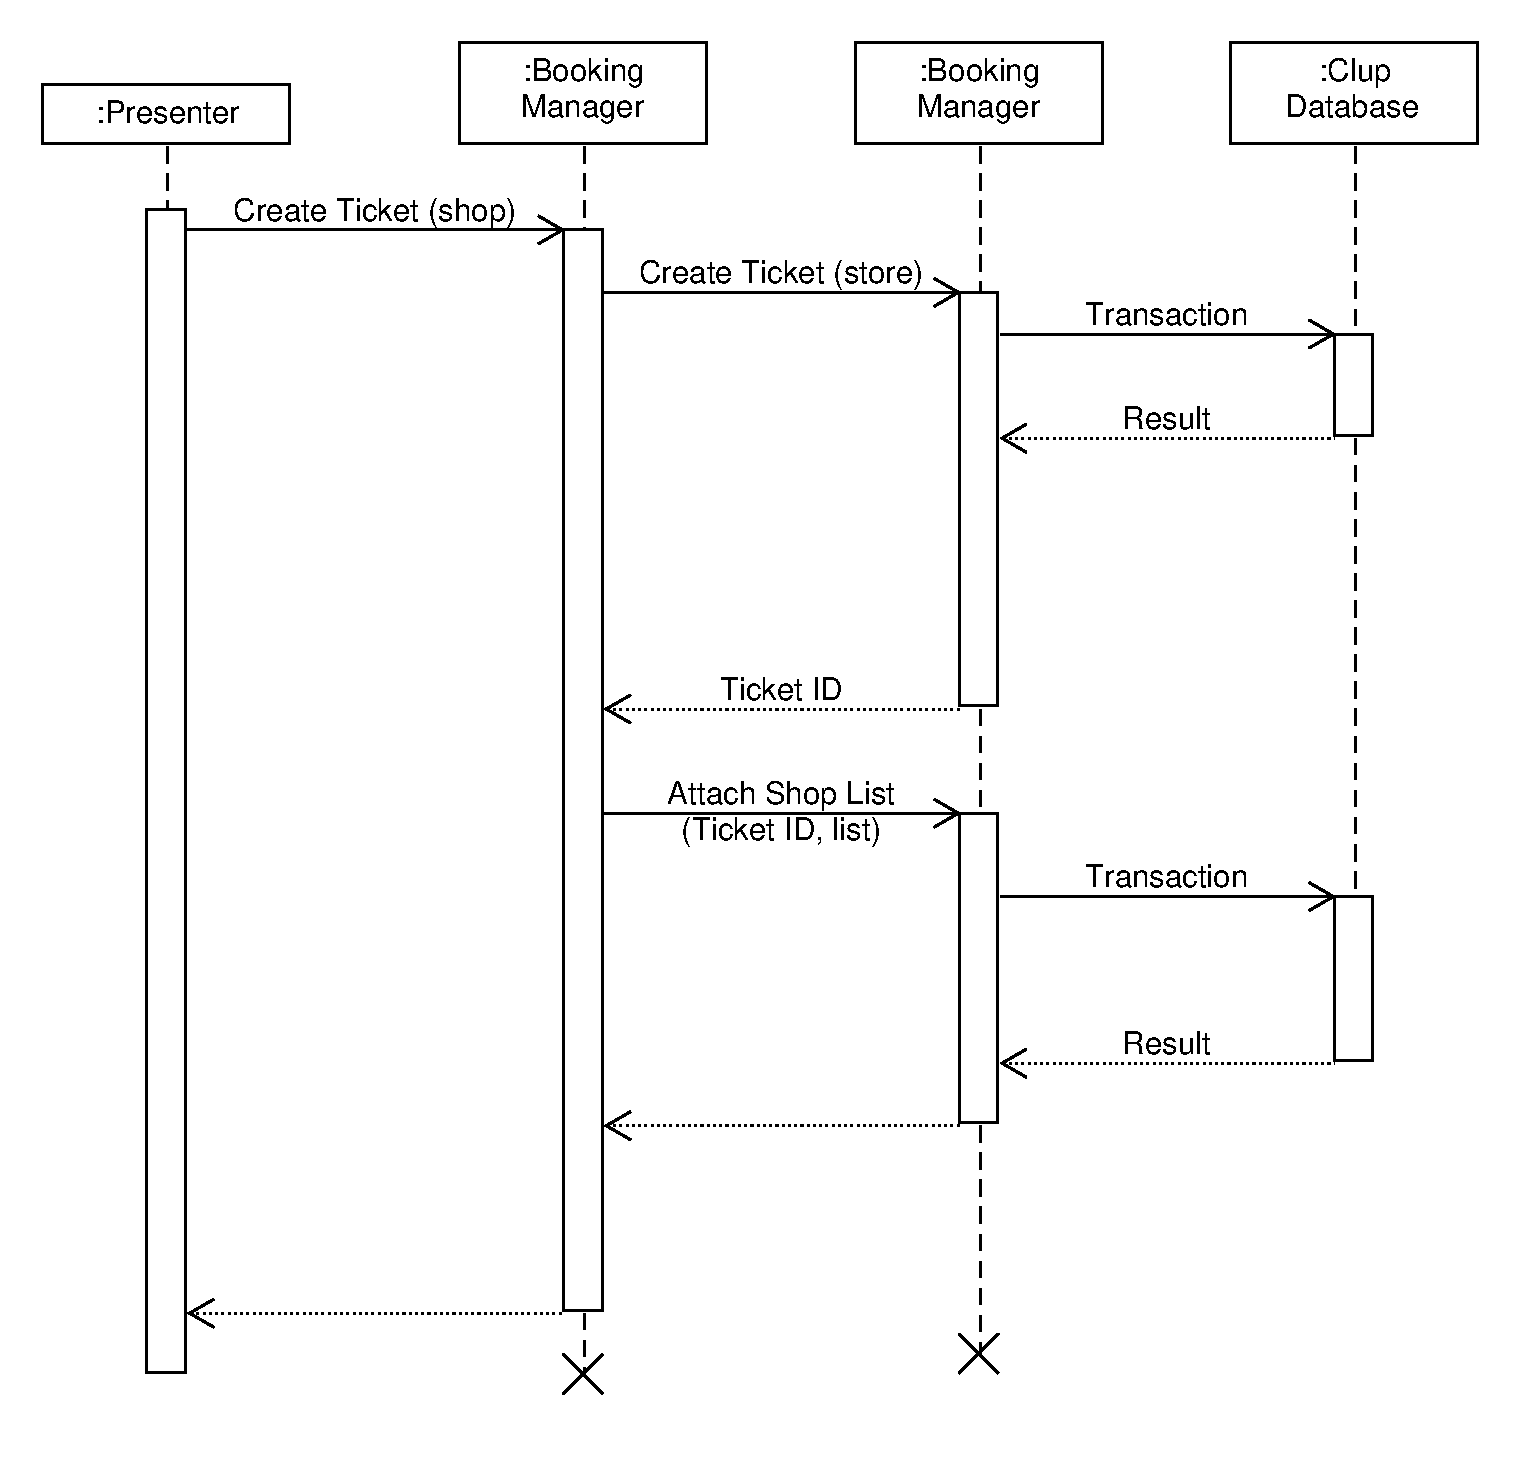
\includegraphics[width=\textwidth]{Images/UML_user_book_visit.pdf}
    \caption{\label{fig:UML_user_book_visit}User books a visit to the store, runtime view}
\end{figure}
The diagram shown in Figure~\ref{fig:UML_user_book_visit} shows how the system behaves when the user requests to book a visit in a store timeslot\footnote{UC 5 - Customer books a visit in a Store, refer to RASD}

The presenter asks the Ticket Controller to generate a reservation; after asking the user the estimated duration of the visit, the Booking Manager component in the CLup Server is called.
When the transaction in the CLup Database has succeeded, the Ticket ID will be returned to the Ticket Controller, which will send the information needed to render the Ticket View to the Presenter, and show it to the user. After the booking is done, the user can optionally attach a shopping list to the reservation he just made. 
\begin{figure}[H]
    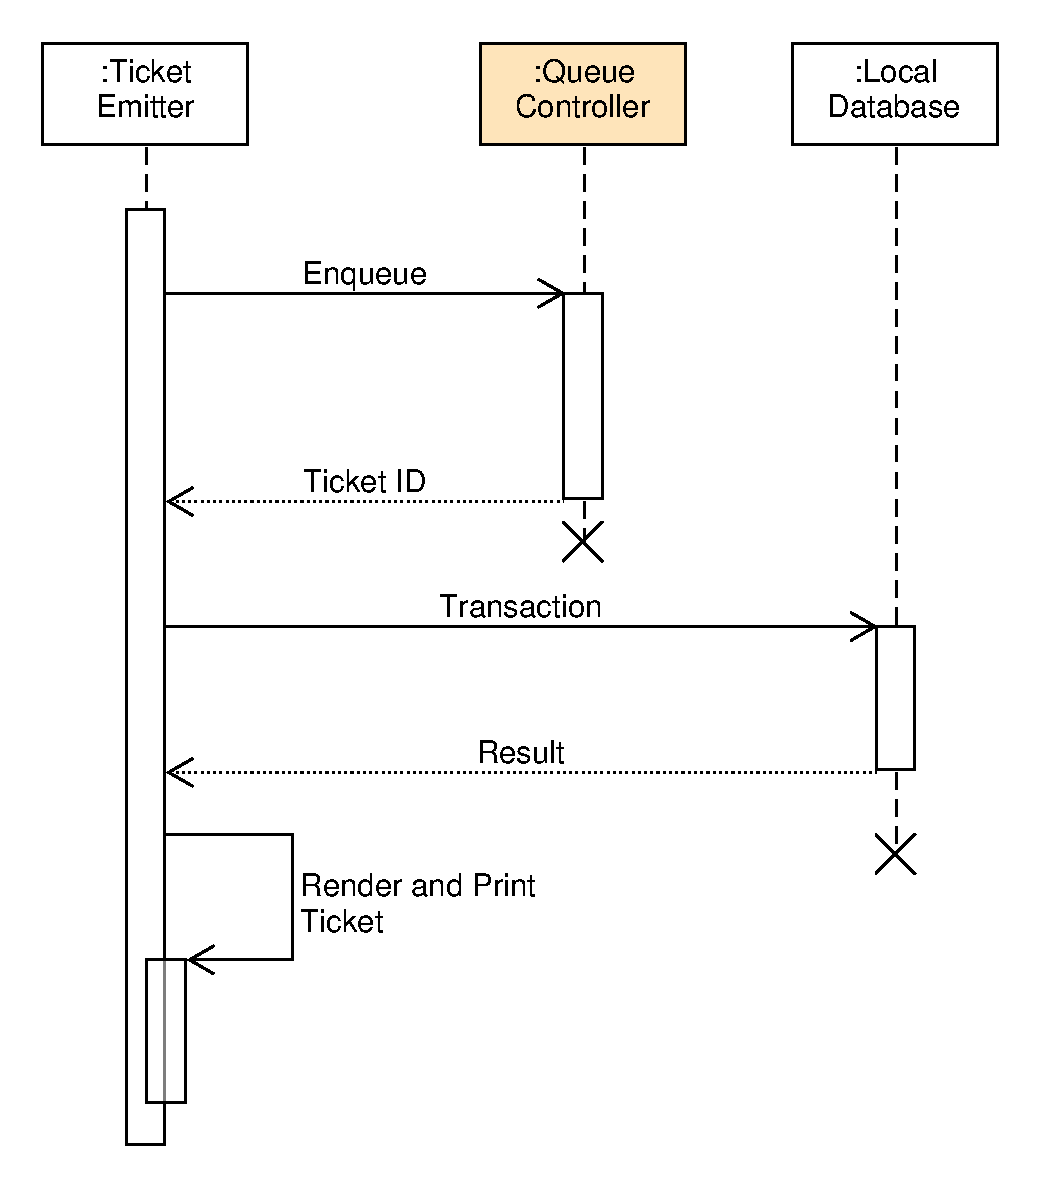
\includegraphics[width=0.7\textwidth]{Images/UML_paper_ticket_sequence.pdf}
    \caption{\label{fig:UML_paper_ticket_sequence}User creates a physical numbered ticket, runtime view}
\end{figure}
The diagram shown in Figure~\ref{fig:UML_paper_ticket_sequence} explains how the system behaves when a customer goes to the store and retrieves a ticket directly from a ticket emitter\footnote{UC 8 -Customer creates a physical numbered ticket, refer to RASD}. Before printing the ticket the emitter adds the customer to the queue, then this ticket is temporarily stored in the store local database. After this the ticket emitter renders the ticket and prints it.
\begin{figure}[H]
    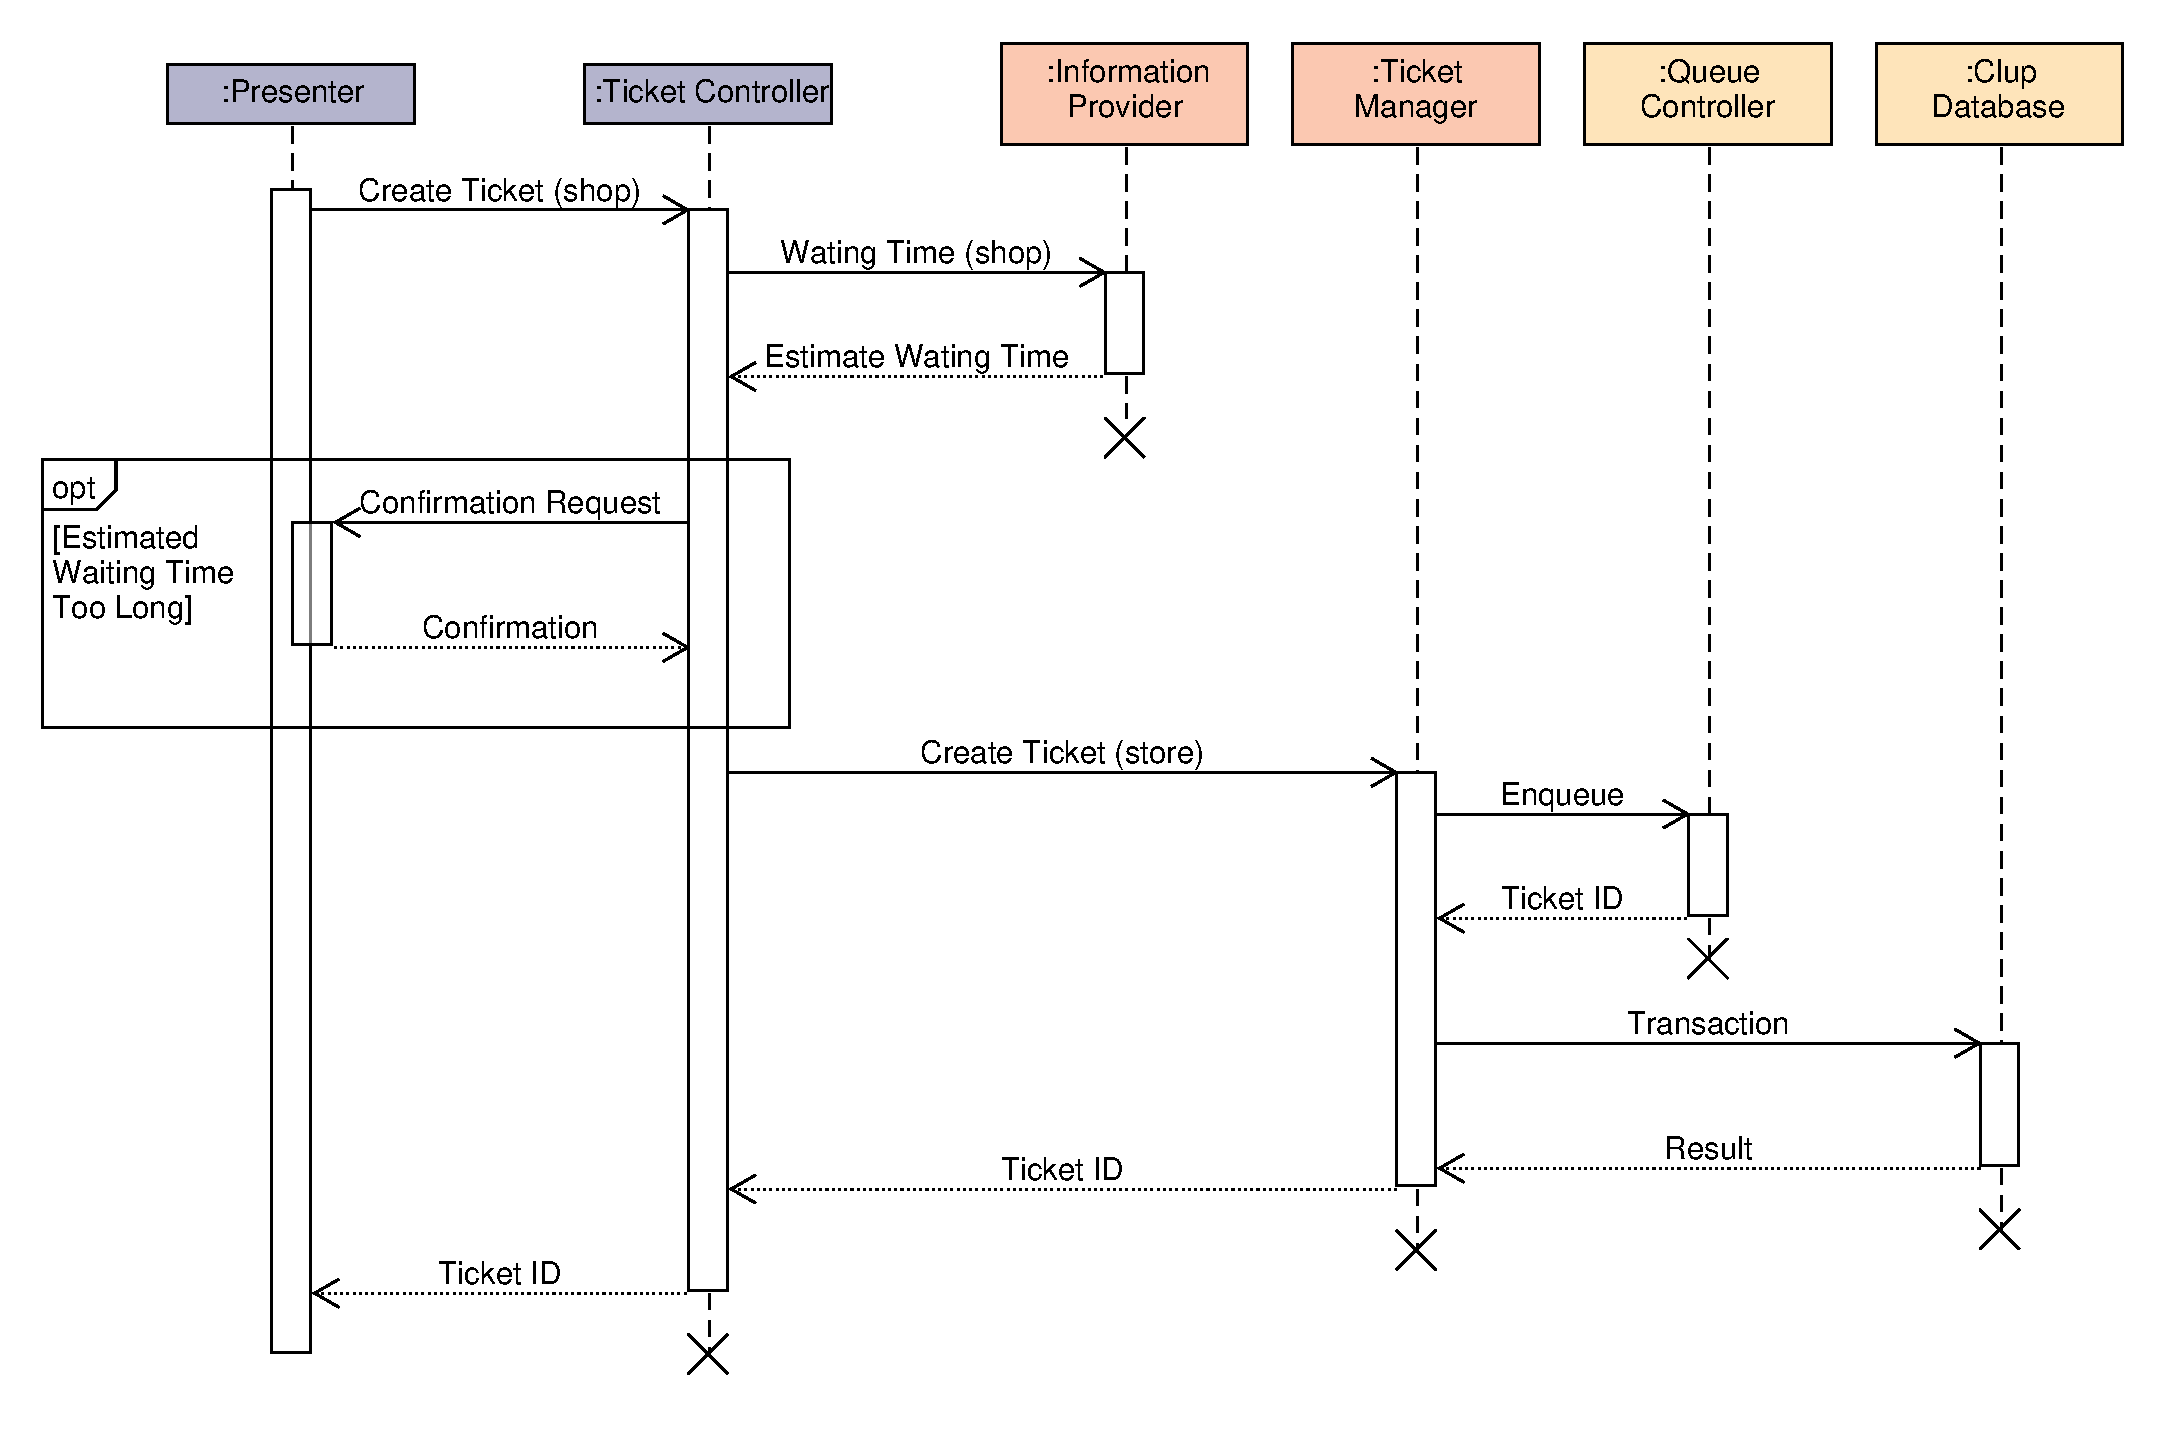
\includegraphics[width=\textwidth]{Images/UML_virtual_ticket_sequence.pdf}
    \caption{\label{fig:UML_virtual_ticket_sequence}User creates a virtual numbered ticket, runtime view}
\end{figure}
The diagram shown in Figure~\ref{fig:UML_virtual_ticket_sequence} illustrates the requests for creating a virtual numbered ticket to enter the store from the User Application\footnote{UC 7 -Customer creates a numbered virtual ticket to enter a store as soon as there is a place available, refer to RASD}. The transaction is initiated when the presenter calls that Ticket Controller, this component at first asks the information provider how much time has the user to wait in queue, if this time is higher than a certain threshold, the user is informed and has to confirm the request. The ticket manager then calls the Ticket Manager that sends an enqueue request to the store Queue Controller. Finally the ticket is saved to the CLup main database.
\begin{figure}[H]
    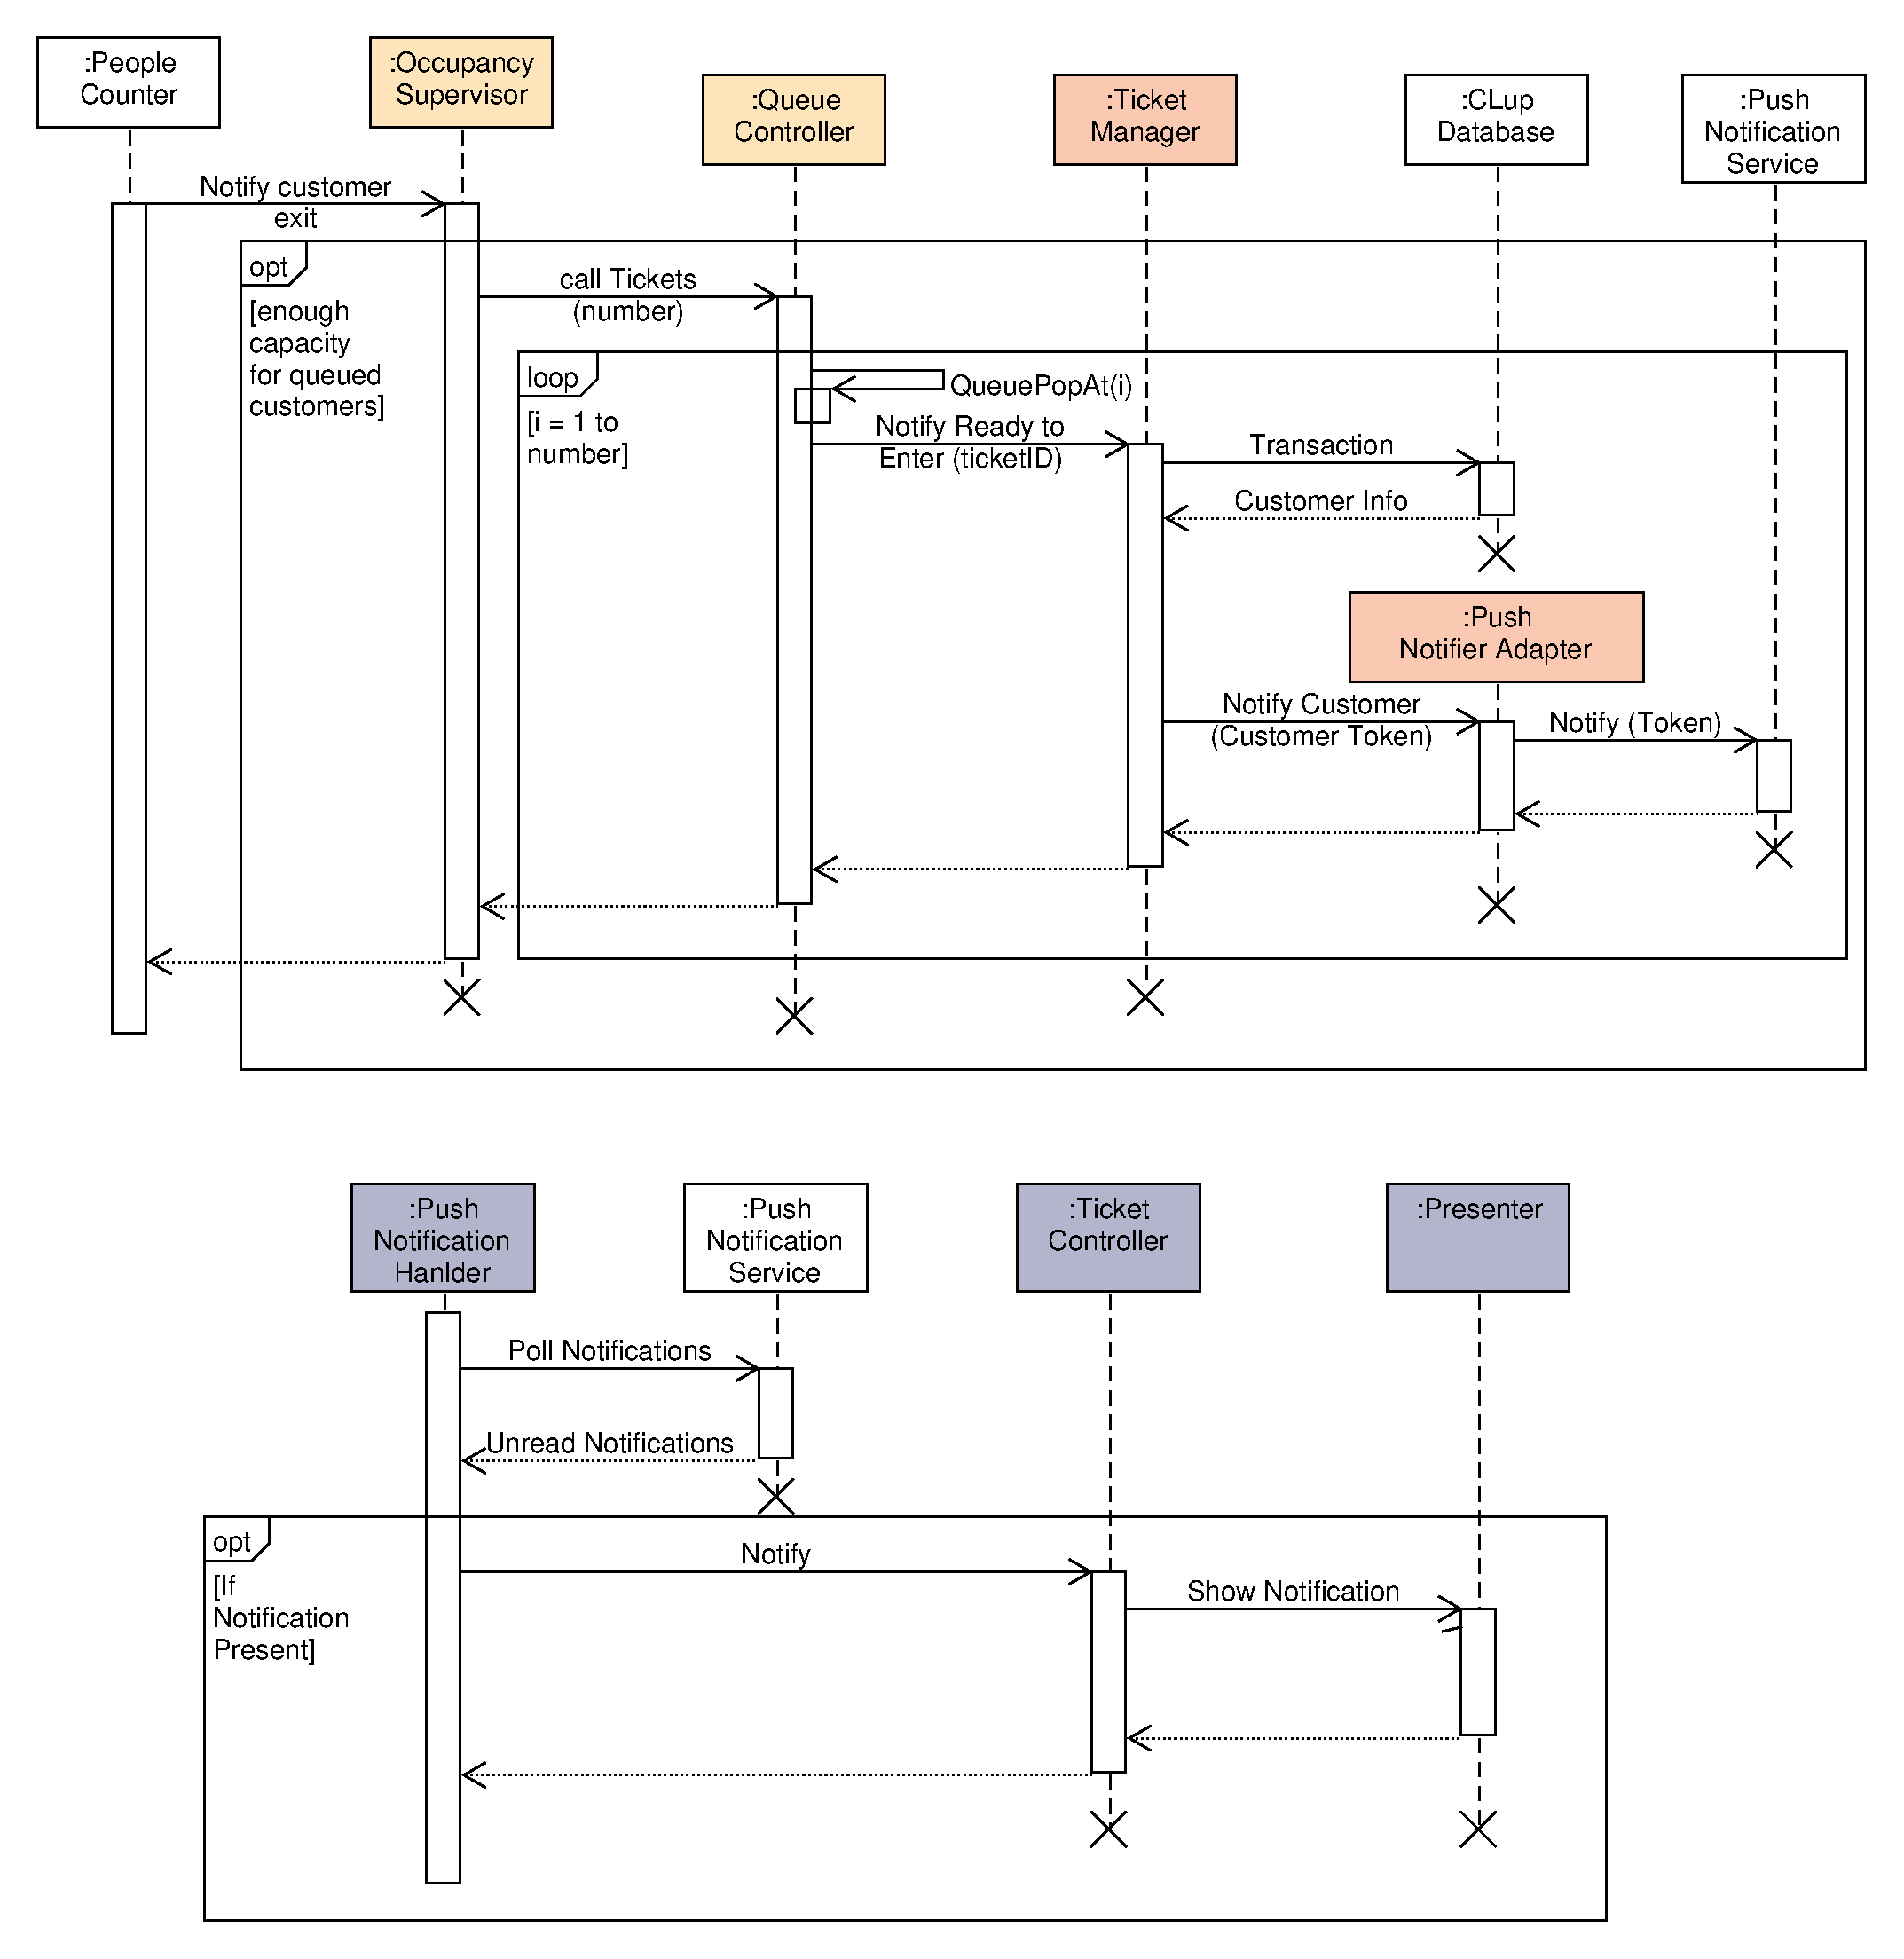
\includegraphics[width=\textwidth]{Images/UML_notification_sequence.pdf}
    \caption{\label{fig:UML_notification_sequence}The store notifies the first customers in queue when they can enter, runtime view}
\end{figure}
The diagram shown in Figure~\ref{fig:fig:UML_notification_sequence} shows the notification process when there is enough capacity for allowing queue customer.

This notification is usually started from a People counter when it detects that someone leaved the store. When this event happens the People Counter calls the occupancy supervisor that calculates how many queued people can enter the store, taking in account the actual occupancy and how many people have booked visits in the oncoming slots. If more than zero people are allowed onto the shop then a number of tickets is popped from the Queue Controller, starting the first. For each popped ticket if that ticket is virtual then the Ticket Manager is called to check the user notification token bound to the ticket and notify that user using the Push Notification Service passing through the adapter component.

The customer device checks periodically the notifications, calling the API provided by the Push Notification service, if a Notification related to CLup is detected the Ticket Controller is called and will call the Presenter that will show the push notification.


\subsection{Component Interfaces}

\clearpage

\definecolor{dkgreen}{rgb}{0,0.6,0}
\definecolor{gray}{rgb}{0.5,0.5,0.5}
\definecolor{mauve}{rgb}{0.58,0,0.82}

\lstset{frame=tb,
    language=Java,
    aboveskip=3mm,
    belowskip=3mm,
    showstringspaces=false,
    columns=flexible,
    basicstyle={\fontsize{10}{11}\ttfamily},
    numbers=none,
    numberstyle=\tiny\color{gray},
    keywordstyle=\color{blue},
    commentstyle=\color{dkgreen},
    stringstyle=\color{mauve},
    breakatwhitespace=true,
}




% interface PushNotificationSenderAPI {
%     ... // Provided by the device OS
% }

% interface PushNotificationReceiverAPI {
%     ... // Provided by the device OS
% }


\begin{lstlisting}
    
    /**
     * It is possible to login using another valid authToken 
     * provided by services like login with a social network account 
     */
    **interfaces AuthenticationInterface, StoreOperatorApplication {
        object LoginResponse(responseType, [authToken]);

        LoginResponse loginWithCredentials(email, password);
        LoginResponse loginWithAnotherAuthService(authenticator, authToken);
    }

    /**
     * The Information Provider yields publicly available data, 
     * so authentication is not required
     */
    interface InformationProviderInterface {
        object StoreCharacteristicsResponse(responseType, 
            [storeID, name, address, gpsPosition, clupStoreSettings]);
        object StoreLiveDataResponse(responseType, [storeID, occupancyData, ...]);

        StoreCharacteristicsResponse getStoreCharacteristics(storeID);
        StoreLiveDataResponse getStoreLiveData(storeID);
        List<storeID> getStoresNearLocation(gpsPosition, kmRadius);
    }

    interface TicketManagerInterface {
        object TicketDetails(ticketNumber, storeID, issueDate, validFrom, validTo);
        object TicketRequestResponse(responseType, [ticketID, TicketDetails]);
        object TicketRevokeResponse(responseType, [ticketID]);
        object TicketDetailsResponse(responseType, [TicketDetails]);

        TicketDetailsResponse getTicketInformation(authToken, ticketID, storeID);
        TicketDetailsResponse getNextIssuableTicketInformation(authToken, storeID);
        TicketRequestResponse requestTicket(authToken, storeID);
        TicketRevokeResponse revokeTicket(authToken, storeID, ticketID);
    }

    interface BookingManagerInterface {
        object BookingDetails(ticketNumber, storeID, issueDate, validFrom, validTo);
        object TimeSlot(timeSlotID, validFrom, validTo, availableReservations);
        object BookingRequestResponse(responseType, [bookingID, BookingDetails]);
        object BookingRevokeResponse(responseType, [bookingID]);
        object TimeSlotsRequestResponse(responseType, [List<TimeSlot>]);

        TimeSlotsRequestResponse getTimeSlots(authToken, storeID, fromDate, toDate);
        BookingRequestResponse requestBooking(authToken, storeID, timeSlotID);
        BookingRevokeResponse revokeBooking(authToken, storeID, timeSlotID);
    }

    /** Both interfaces are provided by the device OS CLup application is running on.
     *  The Notification Adapter transparently handles multiple types 
     */ of Push Notification APIs for the other components.
    interfaces PushNotificationSenderAPI, PushNotificationReceiverAPI {...}

    interface BookingManagerStoreInterface {
        Response cancelBooking(authToken, timeSlotID);
        Response shoplistUpdate(authToken, timeSlotID, shoppingList);
    }

    interface StoreInformationProviderInterface {

    }

    interface TicketManagerStoreInterface {

    }

    // Transactional Database interface, provided by the chosen Database technology
    interface CLupDatabaseInterface {...}

    interface MapAPI {

    }

    interface GPSDataInterface {
        
    }

    interface MapPresenterInterface {
        
    }

    interface ShoplistPresentInterface {

    }

    interface AuthenticationPresenterInterface {
        
    }

    interface BookingCreatorInterface {
        
    }

    *interface ShoplistAttachmentInterface{
        
    }

    *interface TicketNotificationReceiverInterface {
        
    }
    
    interface OccupancyUpdateInterface {

    }

    *interface OccupancyStatisticsInterface {
        
    }

    interface QueueInterface {
        
    }

    interface PeopleCounterInterface {
        
    }

    *interface TicketScreenObserverInterface {
        
    }

    interface AccessControllerInterface{
        
    }

    interface StoreOperatorDataInterface{
        
    }

    interface TicketEmitterInterface{
        
    }


\end{lstlisting}

\subsection{Style Architecture}

% TODO: add section about relevant interfaces and algorithms is pseudocode